\documentclass[xcolor=dvipsnames]{beamer}

\usepackage{lmodern}     
\usepackage{colortbl}   
\usepackage{graphicx}
\usepackage{booktabs}
\usepackage{amsmath}
\usepackage{amssymb}
\usepackage{pifont}
\usepackage{tikz}
\usetikzlibrary{positioning}
\usepackage{amssymb} 
\usepackage{sansmath} 
\sansmath

% --- TEMA E CORES ---
\usetheme{varpa}
\definecolor{udcpink}{RGB}{177,0,114}
\definecolor{udcgray}{RGB}{100,100,100}
\definecolor{ficblue}{RGB}{50,110,118}
\renewcommand{\familydefault}{\sfdefault}

% --- DATOS DA PRESENTACIÓN ---
\title{Aliñamento de imaxes oftalmolóxicas usando representacións neuronais implícitas}
\author[Mateo Amado Ares]{Mateo Amado Ares \\ \vspace{0.5cm} \small{Dirección: José Rouco Maseda e Jorge Novo Buján}}
\date{Xuño de 2025} 


%------------------- INICIO DO DOCUMENTO ----------------------------
\begin{document}

% --- DIAPOSITIVA DE TÍTULO ---
\begin{frame}
    \titlepage
    % NOTAS PARA O PRESENTADOR:
    % - Comeza presentándote e agradecendo a presenza do tribunal.
    % - Menciona o título do teu traballo e os teus directores.
    % - O obxectivo desta primeira diapositiva é establecer unha primeira impresión profesional e segura.
\end{frame}

% --- ÍNDICE XERAL ---
\begin{frame}
    \frametitle{Índice de Contidos}
    \tableofcontents
    % NOTAS PARA O PRESENTADOR:
    % - Presenta brevemente a estrutura da presentación.
    % - Exemplo: "Nesta presentación, comezarei introducindo o problema clínico e os obxectivos do traballo. A continuación, repasarei o contexto tecnolóxico e a nosa metodoloxía. Despois, presentarei os experimentos e os resultados máis relevantes, para finalmente concluír coas achegas principais e as futuras liñas de investigación."
    % - Isto axuda á audiencia a seguir o fío da túa exposición.
\end{frame}

% Con esto hacemos que al entrar en cada sección aparezca el índice
% con la sección actual remarcada. Mantener!
\AtBeginSection[]
{
  \begin{frame}<beamer>
    \frametitle{Tabla de contenidos}
    \tableofcontents[current,currentsubsection]
  \end{frame}
}

\AtBeginSubsection[] {
    \begin{frame}<beamer>
    \frametitle{Tabla de contenidos}
    \tableofcontents[current, currentsubsection]  
    \end{frame}
}

% --- SECCIÓN 1: INTRODUCIÓN E MOTIVACIÓN --- %
\section{Introdución e Motivación}
\begin{frame}
    \frametitle{O Problema Clínico: Aliñamento de Imaxes de Retina}

    \begin{block}{Necesidade Clínica}
        \begin{itemize}
            \item O aliñamento de imaxes de retina é fundamental para:
            \begin{itemize}
                \item Rastrear a progresión de enfermidades como o glaucoma ou a retinopatía diabética.
                \item Fusionar información de distintas fontes, como retinografía e OCT.
            \end{itemize}
            \item O ollo permite a observación directa de tecido neuronal e vasos sanguíneos, clave para o diagnóstico precoz.
        \end{itemize}
    \end{block}

    % \vspace{0.1cm}

    \begin{center}
        \begin{minipage}{0.35\textwidth}
            \centering
            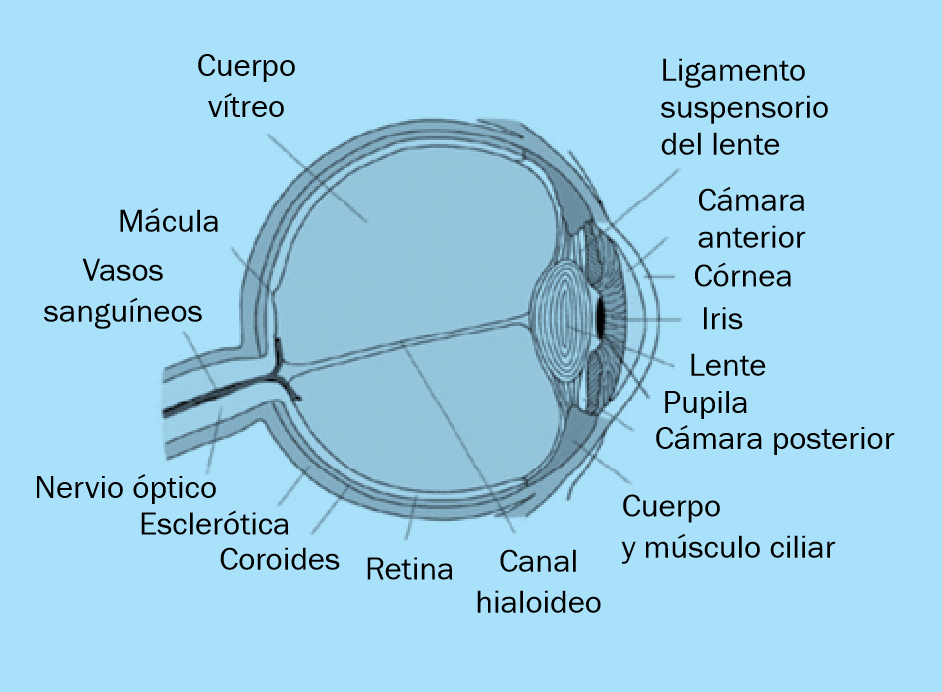
\includegraphics[width=0.95\textwidth]{../imaxes/ojo1.png}
        \end{minipage}
        \hspace{0.05\textwidth}
        \begin{minipage}{0.35\textwidth}
            \centering
            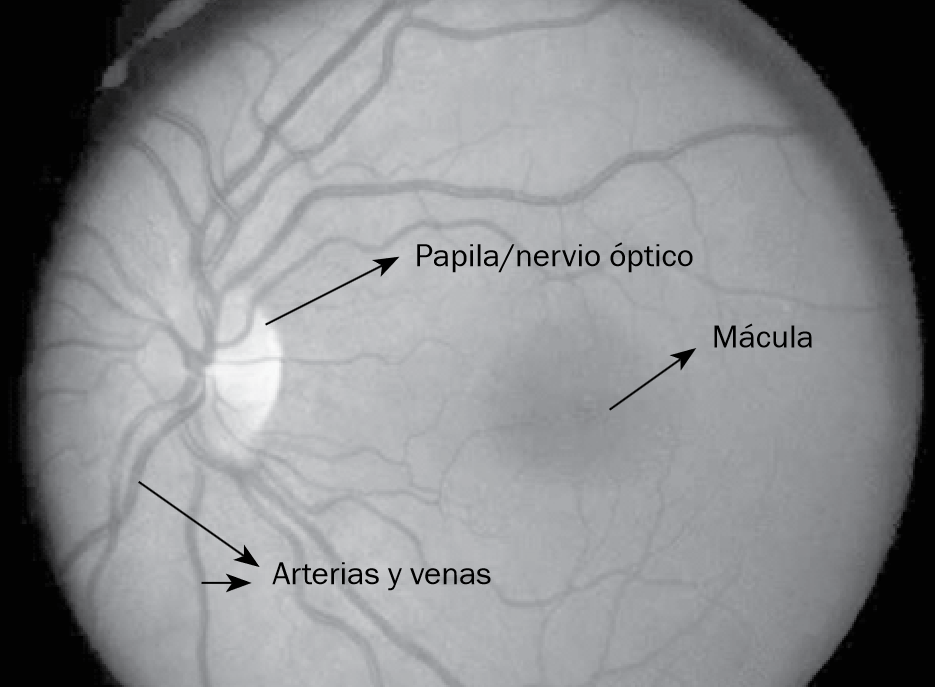
\includegraphics[width=0.95\textwidth]{../imaxes/ojo2.png}
        \end{minipage}
    \end{center}
    % \small{Imaxes do ollo humano, extraídas de \cite{visionyojo}. Á esquerda, vista lateral do ollo anotada. Á dereita, retinografía do ollo anotada.}

    % NOTAS PARA O PRESENTADOR:
    % - Explica a imaxe da dereita: "O obxectivo é deformar unha imaxe móbil para aliñala cunha fixa, como se ve no resultado superposto".
    % - Expón a necesidade clínica: "Isto permite comparar imaxes tomadas en diferentes momentos para ver a evolución dunha enfermidade".
    % - Subliña a importancia do ollo como ferramenta de diagnóstico.
\end{frame}

\begin{frame}
    \frametitle{O Reto do Aliñamento Manual}

    \begin{alertblock}{O Reto}
        O aliñamento manual é un proceso:
        \begin{itemize}
            \item \textbf{Tedioso e lento}: consume tempo dos especialistas.
            \item \textbf{Subxectivo e propenso a erros}: depende do experto.
            \item \textbf{Non escalable}: inviable para grandes volumes de datos.
        \end{itemize}
        \vspace{0.2cm}
        \rightarrow \textbf{A automatización é de gran interese clínico.}
    \end{alertblock}

    \begin{center}
        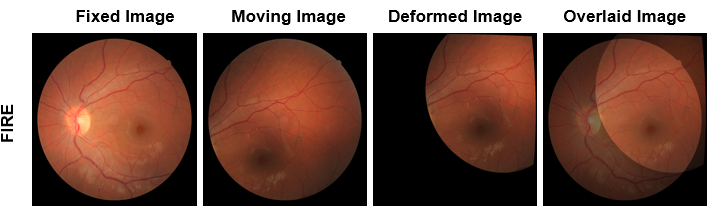
\includegraphics[width=0.75\textwidth]{../imaxes/retin-reg.png}
        
        \small Imaxe fixa, móbil, deformada e resultado superposto.
    \end{center}

    % NOTAS PARA O PRESENTADOR:
    % - Presenta o problema a resolver: "Facer isto a man é lento, difícil e subxectivo. A meta é automatizar o proceso para facelo máis rápido, obxectivo e escalable".
\end{frame}
\begin{frame}
    \frametitle{Obxectivos do Traballo}
    
    O obxectivo principal é \textbf{explorar a viabilidade das Representacións Neuronais Implícitas (INRs) para o aliñamento de imaxes oftalmolóxicas}.
    
    \vspace{0.4cm}
    
    Obxectivos específicos:
    \begin{enumerate}
        \item \textbf{Adaptar o framework IDIR}: Modificar a arquitectura orixinal, pensada para imaxes 4D-CT de pulmóns, para rexistro en 2D de retina.
        \item \textbf{Avaliar o rendemento}: Comparar o método en dous conxuntos de datos:
        \begin{itemize}
            \item \textbf{FIRE}: Imaxes clínicas reais, con variabilidade do mundo real.
            \item \textbf{RFMID}: Imaxes sintéticas con transformacións coñecidas.
        \end{itemize}
        \item \textbf{Analizar a os resultados}: En particular se a activación SIREN ofrece vantaxes para capturar deformacións.
    \end{enumerate}
    
    % NOTAS PARA O PRESENTADOR:
    % - Resume: adaptamos un método, probámolo en dous escenarios e analizamos se SIREN mellora os resultados fronte a ReLU.
\end{frame}

% ------------------- SECCIÓN 2:  Contexto e Estado da Arte ---------------------- %
\section{Contexto e Estado da Arte}

\begin{frame}
    \frametitle{Rexistro Deformable: Campo de Vectores de Deformación}
        
        \begin{block}{Rexistro Deformable}
            Atopar unha transformación non ríxida que mapea cada coordenada $x$ da imaxe móbil á súa localización correspondente na imaxe fixa.
            \begin{itemize}
                \item Modélase como un \textbf{Campo de Vectores de Deformación} (DFV), que indica o desprazamento de cada punto.
                \item Tradicionalmente represéntase o DFV nunha grella discreta de píxeles. Isto ten limitacións de resolución e memoria.
            \end{itemize}
        \end{block}

        \begin{minipage}{\textwidth}
            \centering
            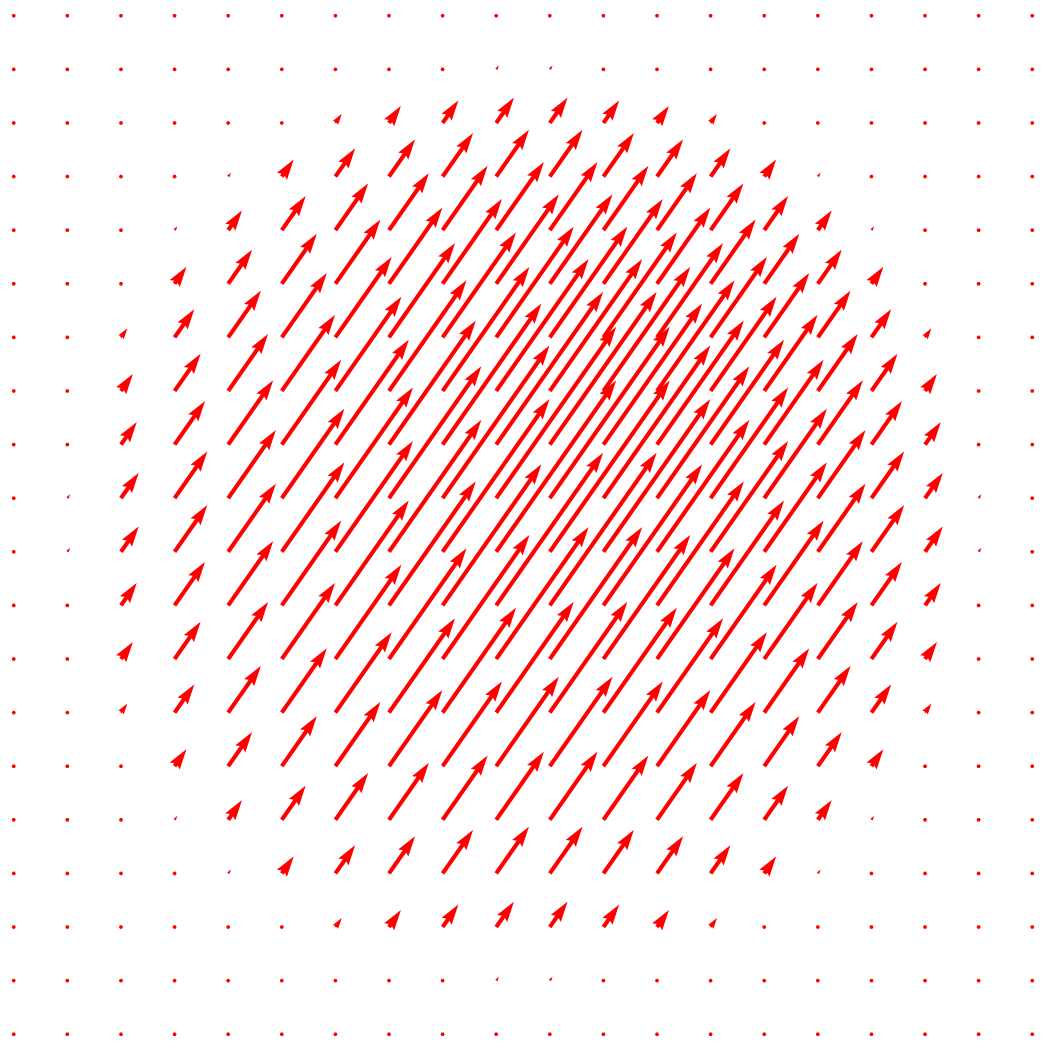
\includegraphics[width=0.22\linewidth]{../imaxes/dfv_arrows.png}
            \hspace{2cm}
            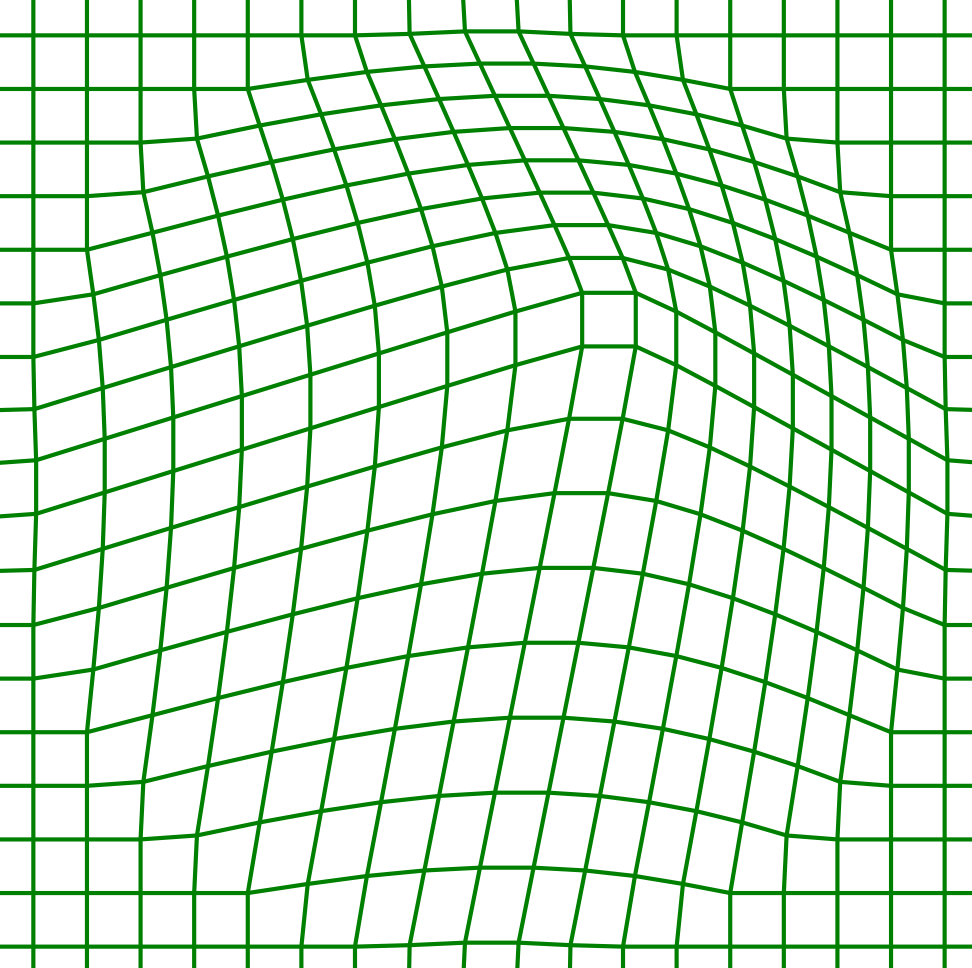
\includegraphics[width=0.22\linewidth]{../imaxes/dfv_grid.png}
        \end{minipage}
    \end{frame}

\begin{frame}
    \frametitle{Representacións Neuronais Implícitas (INRs)}
    \begin{block}{Representacións Neuronais Implícitas (INRs)}
        En lugar dunha grella, representamos a transformación como unha \textbf{función continua}, parametrizada polos pesos dunha rede neuronal (MLP).
        \begin{itemize}
            \item \textbf{Entrada}: Coordenada $(x, y)$.
            \item \textbf{Saída}: Vector de desprazamento $(dx, dy)$.
            \item \textbf{Vantaxes clave}:
            \begin{itemize}
                \item \textbf{Independencia da resolución}: A función é continua, non depende do tamaño da imaxe.
                \item \textbf{Gradientes analíticos}: Permite calcular derivadas exactas da deformación, crucial para unha regularización precisa.
            \end{itemize}
        \end{itemize}
    \end{block}
\end{frame}
  
    % NOTAS PARA O PRESENTADOR:
    % - Empeza coa imaxe: "Para aliñar as imaxes, necesitamos calcular un campo de vectores de deformación, ou DFV. Como se ve á dereita, este campo nos di como torcer e estirar unha grella para que coincida coa outra imaxe."
    % - Explica o enfoque tradicional: "A forma clásica de facer isto é almacenar estes vectores nunha grella de píxeles. Pero isto consume moita memoria e a precisión está limitada pola resolución da grella."
    % - Introduce o cambio de paradigma coas INRs: "O noso enfoque é diferente e máis moderno. En lugar dunha grella, usamos unha pequena rede neuronal para que *aprenda a función* matemática da deformación. Esta rede toma como entrada unha coordenada (x,y) e devolve o desprazamento (dx,dy) para ese punto."
    % - Destaca as dúas vantaxes fundamentais: "Isto ten dúas vantaxes enormes. Primeiro, como é unha función continua, é independente da resolución da imaxe. Segundo, e máis importante, podemos calcular as súas derivadas de forma exacta e analítica. Isto é un salto cualitativo sobre as aproximacións numéricas dos métodos baseados en grellas e, como veremos, permítenos usar 'regras' ou regularizacións moito máis sofisticadas."

    \begin{frame}
        \frametitle{O Problema do Sesgo Espectral}

        \begin{block}{Limitación das Redes con ReLU}
            As funcións de activación lineais coma ReLU presentan un \textbf{sesgo espectral} cara funcións de baixa frecuencia (tranformacións globais e ríxidas), e teñen dificultades para representar detalles finos e cambios locais.
            
            \vspace{0.3cm}
            No contexto do rexistro de retinas, isto é problemático porque os detalles de alta frecuencia son críticos para un aliñamento preciso.
        \end{block}

        % NOTAS PARA O PRESENTADOR:
        % - Expón o problema fundamental das redes estándar: "Por que non usar unha rede normal con ReLU? O problema é o chamado 'sesgo espectral'."
        % - Explica: "ReLU aprende ben cousas borrosas, pero mal detalles nítidos. No noso caso, iso é un problema."
    \end{frame}

    \begin{frame}
        \frametitle{SIREN (Sinusoidal Representation Networks)}

        \begin{alertblock}{A Solución: }
            SIREN utiliza a función seno como activación para superar o sesgo espectral e modelar detalles finos.
            
            \centering
            \[
            f(x) = \sin(ax + b), \quad \text{con} \quad a, b \in \mathbb{R}
            \]
            
            \begin{itemize}
                \item \textbf{Ideal para sinais complexos}: Permite representar detalles de alta frecuencia e as súas derivadas.
                \item \textbf{Infinitamente diferenciable}: A diferenza de ReLU, a función seno pode derivarse cantas veces sexa necesario, permitindo regularizacións de orde superior.
            \end{itemize}
        \end{alertblock}

        % NOTAS PARA O PRESENTADOR:
        % - Presenta SIREN como solución: "SIREN usa activación seno, ideal para detalles finos."
        % - Destaca a diferenciabilidade: "Isto permite regularizacións máis potentes, como veremos a continuación."
    \end{frame}


\begin{frame}
\frametitle{Estado da Arte: Métodos Clásicos}
\begin{block}{Rexistro baseado en características (FBR)}
Identifican, describen e emparellan características salientables entre imaxes.
\begin{itemize}
% \item Detectan, describen e emparellan puntos característicos entre imaxes.
\item Robustos ante variacións locais e cambios de modalidade.
% \item \textbf{Exemplos en Retina}: \textbf{VOTUS}, que representa árbores vasculares como grafos, e \textbf{REMPE}, que modela a forma 3D do ollo.
\end{itemize}
\end{block}

\begin{block}{Rexistro baseado en intensidade (IBR)}
    Comparan directamente os valores de intensidade dos píxeles mediante unha métrica de similitude e optimizan iterativamente a transformación.
    \begin{itemize}
        \item  Non requiren a extracción de características explícitas.
        \item  Máis sensibles a ruido e variacións de iluminación ou estrutura.
    \end{itemize}
\end{block}



% NOTAS PARA O PRESENTADOR:
% - "Tradicionalmente, o rexistro facíase de dúas formas."
% - "A primeira, baseada en características, é como buscar puntos de referencia comúns, como cruces de vasos sanguíneos. Métodos como VOTUS ou REMPE son moi precisos pero computacionalmente custosos."
% - "A segunda, baseada en intensidade, compara directamente os valores dos píxeles, buscando a transformación que fai as imaxes o máis parecidas posible. O noso método inscríbese nesta segunda familia."

\end{frame}

\begin{frame}
\frametitle{Estado da Arte: Métodos de Aprendizaxe Profunda}

\begin{block}{Dúas Estratexias Principais}
    As redes neuronais abordan o rexistro de dúas formas:
    \begin{itemize}
        \item \textbf{Aprendizaxe Extremo a Extremo (\textit{End-to-End})}: Predí directamente a deformación a partir dun par de imaxes.
        % \begin{itemize}
        %     \item Adestramento \textbf{non supervisado}, optimizando a similitude das imaxes. Moi rápido na inferencia.
        % \end{itemize}
        \item \textbf{Mellora de Métodos Clásicos}: Empréganse redes para substituír compoñentes das metodoloxías clásicas.
        % \begin{itemize}
        %     \item \textbf{SuperPoint} aprende a detectar puntos de interese e \textbf{SuperGlue} a emparellalos.
        % \end{itemize}
    \end{itemize}
\end{block}
    
\begin{alertblock}{O noso enfoque: Modelo de Transformación}
    O noso método, IDIR, aprende unha representación implícita da transformación parametrizada nos pesos da rede neuronal para cada par de imaxes.
\end{alertblock}

% NOTAS PARA O PRESENTADOR:
% - "Hoxe en día, o deep learning domina o rexistro de dúas maneiras: ou redes xigantes que aprenden toda a tarefa de golpe, ou redes máis pequenas que melloran os métodos clásicos."
% - "O noso enfoque é distinto. Adestramos unha rede pequena e nova para cada par de imaxes, para que aprenda a función matemática exacta da deformación necesaria."

\end{frame}


\begin{frame}
\frametitle{Estado da Arte en Retinografías}
\begin{block}{Desafíos}
    Rexistro difícil por deformacións non ríxidas, baixo solapamento e variacións de iluminación e anatomía.
\end{block}
\begin{alertblock}{Solucións Actuais e Contribución}
    \begin{itemize}
        \item \textbf{Tendencia Actual: Métodos Híbridos}: Combinan deep learning e algoritmos clásicos para lograr precisión e velocidade.
        \item \textbf{A Nosa Contribución}: Primeira aplicación de Representacións Neuronais Implícitas (INRs) ao rexistro de retinografías, adaptando o framework IDIR a este dominio.
    \end{itemize}
\end{alertblock}

% NOTAS PARA O PRESENTADOR:
% - "O rexistro de retinas é un problema particularmente difícil."
% - "Os métodos máis punteiros hoxe en día son híbridos, combinando o mellor de varios mundos. Son rápidos e precisos."
% - "Aquí é onde o noso traballo destaca: estamos a abrir un novo camiño. Somos os primeiros en investigar se as Representacións Neuronais Implícitas son unha solución viable para este problema."

\end{frame}

% ------------------- SECCIÓN 3:  Metodoloxía ---------------------- %
\section{Metodoloxía Proposta}

% Slide 1: Framework IDIR Adaptado - Esquema do Proceso
\begin{frame}
    \frametitle{Framework IDIR: Esquema do Proceso}
    
    \begin{block}{Optimización por Par de Imaxes}
        A metodoloxía de IDIR adestra unha nova rede para cada par de imaxes (Fixa $F$ e Móbil $M$).
    \end{block}
    
    \centering
    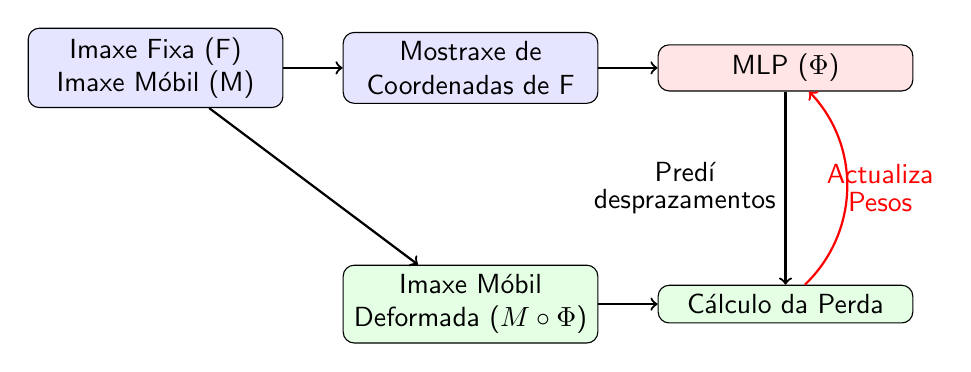
\begin{tikzpicture}
        \node[draw, rectangle, rounded corners, fill=blue!10, text width=3cm, align=center] (in) at (0,3) {Imaxe Fixa (F) \\ Imaxe Móbil (M)};
        \node[draw, rectangle, rounded corners, fill=blue!10, text width=3cm, align=center] (coords) at (4,3) {Mostraxe de Coordenadas de F};
        \node[draw, rectangle, rounded corners, fill=red!10, text width=3cm, align=center] (mlp) at (8,3) {MLP ($\Phi$)};
        
        \node[draw, rectangle, rounded corners, fill=green!10, text width=3cm, align=center] (warp) at (4,0) {Imaxe Móbil Deformada ($M \circ \Phi$)};
        \node[draw, rectangle, rounded corners, fill=green!10, text width=3cm, align=center] (loss) at (8,0) {Cálculo da Perda};
        
        \draw[->, thick] (in) -- (coords);
        \draw[->, thick] (coords) -- (mlp);
        \draw[->, thick] (mlp) -- (loss);
        \draw[->, thick] (in) -- (warp);
        \draw[->, thick] (warp) -- (loss);
        % Add labels on both sides of the arrow from mlp to loss
        \path (mlp) -- (loss) coordinate[pos=0.5] (midpoint);
        \node[left=0cm of midpoint] {\shortstack{Predí\\desprazamentos}};
        \node[right=0.4cm of midpoint, text=red] {\shortstack{Actualiza\\Pesos}};

        % Feedback arrow
        \draw[->, thick, red] (loss) to[bend right=45] (mlp);
    \end{tikzpicture}
    % NOTAS PARA O PRESENTADOR:
    % - Explica o diagrama de fluxo paso a paso.
    % - Fai fincapé no punto clave: "É importante destacar que este é un proceso de 'optimización por instancia'. Adestramos unha rede nova e pequena para cada par de imaxes. Isto diferéncianos da maioría de métodos de deep learning que requiren miles de exemplos para adestrar un único modelo xigante. O noso enfoque é máis lento na inferencia, pero non necesita grandes bases de datos anotadas, que son moi caras e difíciles de conseguir no ámbito médico".[1, 3]
\end{frame}

% Slide 2: Framework IDIR Adaptado - Función de Perda
\begin{frame}
    \frametitle{Framework IDIR: Función de Perda}
    
    \begin{block}{Función de Perda}
        A rede optimízase para minimizar unha perda combinada:
        \vspace{0.4cm}
        \centering
        $\hat{\Phi} = \operatorname*{Arg\,min}_{\Phi} L_{data}(M \circ \Phi, F) + \alpha L_{reg}(\Phi)$
        \vspace{0.4cm}
        \begin{itemize}
            \item $\mathcal{L}_{datos}$: Mide a similitude entre a imaxe fixa e a móbil deformada (e.g., NCC).
            \item $\mathcal{L}_{reg}$: Penaliza as deformacións non realistas para garantir a suavidade.
        \end{itemize}
    \end{block}
    
    % NOTAS PARA O PRESENTADOR:
    % - Explica as dúas partes da función de perda: "A perda ten dúas partes: unha que mide o parecidas que son as imaxes (L_datos), e outra que mide o 'realista' que é a deformación (L_reg)."
    % - Resume o proceso: "Calculamos esta perda e usamos para actualizar os pesos da rede, repetindo ata converxer."
\end{frame}

% Slide 1: Por que é necesaria a regularización?
\begin{frame}
    \frametitle{Framework IDIR: Regularización}
    
    \begin{block}{Problema:}
        O rexistro de imaxes é un \textit{"ill-posed problem"}: existen moitas deformacións que poden facer que as imaxes se parezan, pero a maioría non son solucións correctas (non fisicamente realistas).
        \vspace{0.2cm}
        
        \textbf{A regularización engade coñecemento previo físico} para restrinxir o espazo de solucións posibles.
    \end{block}
    
    \begin{columns}
        \begin{column}{0.6\textwidth}
            \centering
            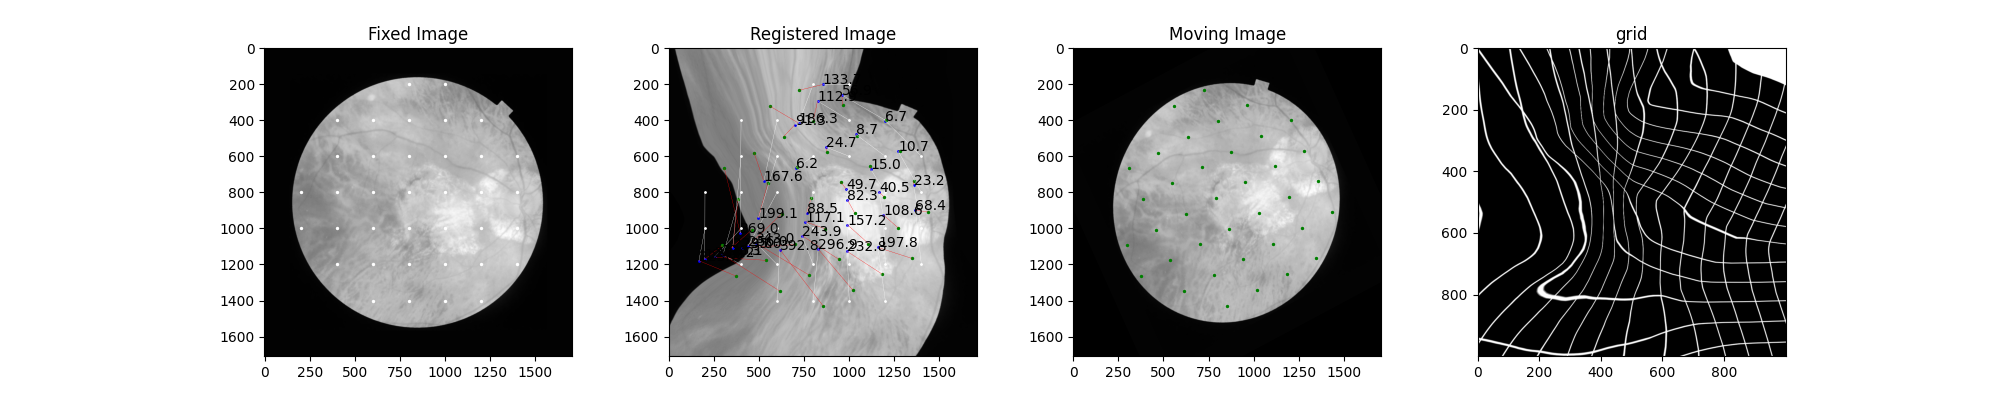
\includegraphics[width=\textwidth]{../imaxes/reg_examples/no_reg_example.png}
            \small{Sen regularización: pregamentos non físicos.}
        \end{column}
        \begin{column}{0.6\textwidth}
            \centering
            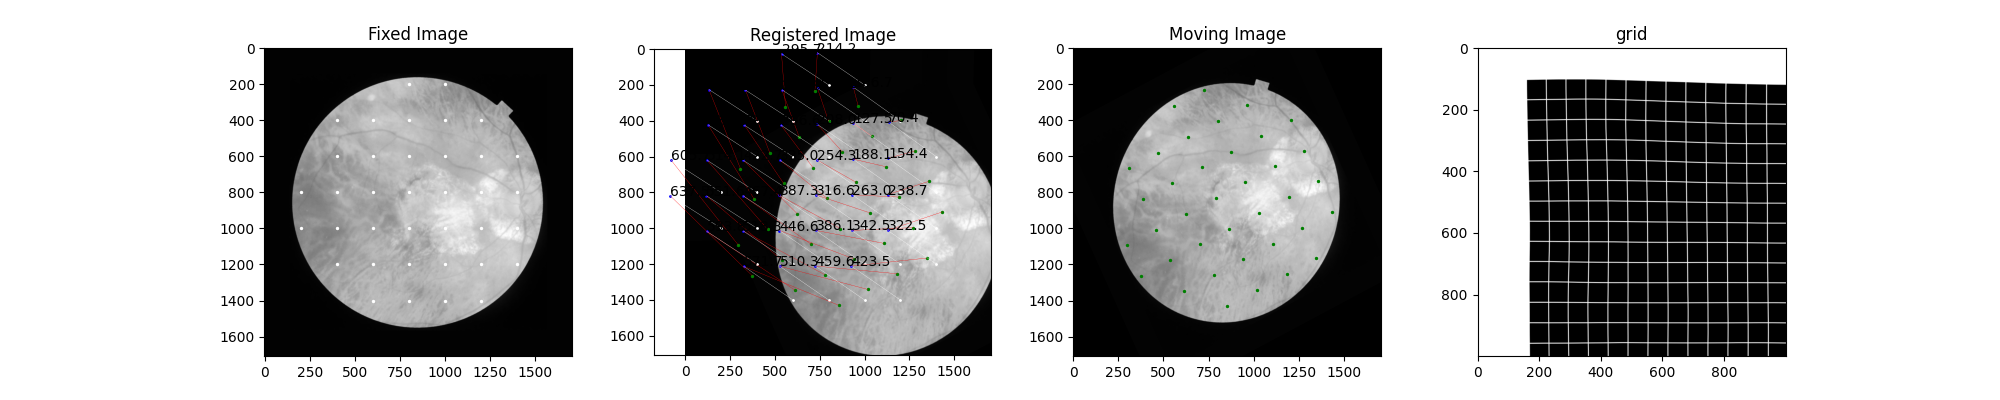
\includegraphics[width=\textwidth]{../imaxes/reg_examples/too_much_reg_example.png}
            \small{Exceso de regularización: deformación demasiado ríxida.}
        \end{column}
    \end{columns}
    
    % NOTAS PARA O PRESENTADOR:
    % - Explica que sen regularización, a rede pode atopar solucións matematicamente válidas pero absurdas fisicamente.
    % - Mostra visualmente os dous extremos: caos sen regularización e rixidez excesiva con demasiada regularización.
\end{frame}

% Slide 2: Regularizadores utilizados
% \begin{frame}
%     \frametitle{Framework IDIR: Regularizadores utilizados}
%         \begin{itemize}
%         \item \textbf{Hiperelástico}: Modela o comportamento elástico dos tecidos. Penaliza estiramentos e compresións non realistas para preservar a área local.
%         \vspace{0.2cm}
%         \item \textbf{Enerxía de Flexión (\textit{Bending Energy})}: Asegura a suavidade da deformación penalizando as segundas derivadas. Evita "esquinas" ou cambios bruscos na deformación.
%         \vspace{0.2cm}
%         \item \textbf{Xacobiano (\textit{Jacobian})}: Controla a distorsión local da área. Garante que a deformación non colapse áreas locais, mantendo a continuidade.
%     \end{itemize}
    

    
%     % NOTAS PARA O PRESENTADOR:
%     % - Introduce os regularizadores como regras físicas que guían a rede.
%     % - Destaca que a arquitectura SIREN permite usar regularizacións baseadas en derivadas de orde superior, mellorando o control físico da deformación.
% \end{frame}

\begin{frame}
\frametitle{Framework IDIR: Regularizador Xacobiano}

\begin{itemize}
    \item Controla a distorsión local da área e prevé pregamentos (\textit{folding}) non realistas na deformación, evitando compresións ou estiramentos extremos.
    \vspace{0.3cm}
    \item \textbf{Mecanismo}: Penaliza as desviacións do determinante da matriz Xacobiana ($\det \nabla \Phi$) respecto do valor 1.
    \begin{itemize}
        \item Un determinante próximo a 1 preserva a área local.
        \item Un determinante negativo ou cero indica un pregamento da malla, o que invalida a transformación.
    \end{itemize}
\end{itemize}

\vfill % Empurra o contido seguinte cara abaixo

\centering
% \textbf{Formulación 2D}
% \vspace{0.2cm}
$$
S^{\text{jac}}[\Phi] = \int_{\Omega} \left| 1 - \det(\nabla \Phi) \right| \, dx \, dy
$$

% NOTAS PARA O PRESENTADOR:
% - Explicar que o determinante do Xacobiano mide como cambia a área localmente.
% - Imaxinar unha pequena cuadrícula na imaxe orixinal; este regularizador tenta que esa cuadrícula non se colapse nin se estire de forma desmedida.

\end{frame}




\begin{frame}
\frametitle{Framework IDIR: Regularizador Hiperelástico}

\begin{itemize}
    \item \textbf{Mecanismo}: Combina termos que penalizan a variación da lonxitude dos vectores de desprazamento e as distorsións de área.
     \begin{itemize}
        \item O termo $|\nabla u|^2$ controla o estiramento.
        \item O termo co cofactor ($\text{cof}$) controla a deformación da área.
     \end{itemize}
    \vspace{0.3cm}
    \item É un regularizador máis xeral que engloba propiedades do Xacobiano e impón unha certa suavidade.
\end{itemize}

\vfill % Empurra o contido seguinte cara abaixo

\centering
% \textbf{Formulación 2D}
% \vspace{0.2cm}
$$
S^{\text{hyper}}[\Phi] = \int_{\Omega} \left[ \frac{1}{2} \alpha_l |\nabla u|^2 + \alpha_a \varphi_c (\text{cof} \nabla \Phi) \right] dx \, dy
$$
\vspace{0.2cm}
\small
con
$$
\varphi_c(C) = \sum_{i=1}^2 \max \left\{ \sum_{j=1}^2 C_{ji}^2 - 1, 0 \right\}^2
$$

% NOTAS PARA O PRESENTADOR:
% - Describir este regularizador como unha "lei física" que lle impoñemos á rede.
% - Mencionar que os hiperparámetros α permiten axustar a "rixidez" do material simulado.

\end{frame}



\begin{frame}
\frametitle{Framework IDIR: Regularizador de Enerxía de Flexión}

\begin{itemize}
    \item Evita cambios bruscos na curvatura do campo de desprazamento, o que se traduce en transformacións visualmente máis suaves e continuas.
    \vspace{0.3cm}
    \item Penaliza a magnitude das segundas derivadas parciais do campo de deformación ($\Phi$) en todo o dominio.
    \vspace{0.3cm}
\end{itemize}

% \begin{alertblock}{Vantaxe SIREN}
%     O cálculo eficiente e analítico deste regularizador só é posible porque as redes \textbf{SIREN son infinitamente diferenciables}. Arquitecturas baseadas en ReLU non poden usar este termo, xa que a súa segunda derivada é cero en case todos os puntos.
% \end{alertblock}


\vfill % Empurra o contido seguinte cara abaixo

\centering
% \textbf{Formulación 2D}
% \vspace{0.2cm}
$$
S^{\text{bending}}[\Phi] = \frac{1}{8} \int_{\Omega} \left[ \left( \frac{\partial^2 \Phi}{\partial x^2} \right)^2 + \left( \frac{\partial^2 \Phi}{\partial y^2} \right)^2 + 2 \left( \frac{\partial^2 \Phi}{\partial x \partial y} \right)^2 \right] dx \, dy
$$

% NOTAS PARA O PRESENTADOR:
% - Este é o punto máis importante que xustifica o uso de SIREN.
% - Resaltar que esta capacidade de calcular derivadas de orde superior de forma analítica é o que permite un control físico tan preciso da deformación.

\end{frame}

\begin{frame}
\frametitle{Consideracións sobre a Regularización}

\begin{itemize}
    \item \textbf{Balance da regularización}: É crucial atopar un equilibrio no peso dos termos de regularización.

    \vspace{0.4cm}
    \item \textbf{Custo computacional}: A regularización incrementa significativamente o tempo de cómputo, xa que require calcular gradientes adicionais por época.
    % \begin{itemize}
    %     \item Sen regularización: 1 pasada de retropropagación.
    %     \item Con Xacobiano: 3 pasadas.
    %     \item Con Hiperelástico: 4 pasadas.
    %     \item Con Enerxía de Flexión: 7 pasadas.
    % \end{itemize}
\end{itemize}

\vfill

\begin{alertblock}{Vantaxe SIREN}
    O cálculo de regularizadores de orde superior (como a Enerxía de Flexión) de forma eficiente e analítica só é posible porque as redes \textbf{SIREN son infinitamente diferenciables}. Arquitecturas baseadas en ReLU non poden usar este termo, xa que a súa segunda derivada é cero en case todos os puntos.
\end{alertblock}

% NOTAS PARA O PRESENTADOR:
% - Usar esta diapositiva para resumir as implicacións prácticas de usar regularización.
% - Concluír enfatizando que SIREN non só permite, senón que fai computacionalmente factible, o uso de modelos físicos avanzados para guiar o rexistro de imaxes.

\end{frame}


% ------------------- SECCIÓN 4: EXPERIMENTOS E RESULTADOS ---------------------- %
% \section{Experimentos e Resultados}

\begin{frame}
    \frametitle{Datasets Utilizados}

    \begin{columns}
        \begin{column}{0.5\textwidth}
            \begin{block}{FIRE}
                \begin{itemize}
                    \item 134 pares de imaxes \textbf{clínicas reais}.
                    \item Diferentes graos de variacións en iluminación, patoloxías e superposición.
                \end{itemize}
            \end{block}
        \end{column}
        \begin{column}{0.5\textwidth}
            \begin{block}{RFMID}
                \begin{itemize}
                    \item Xeramos pares de imaxes aplicando transformacións xeométricas \textbf{coñecidas e controladas}.
                    \item Sen variacións de aparencia.
                \end{itemize}
            \end{block}
        \end{column}
    \end{columns}

    \vspace{0.1cm}

    \begin{center}
        \begin{minipage}{0.35\textwidth}
            \centering
            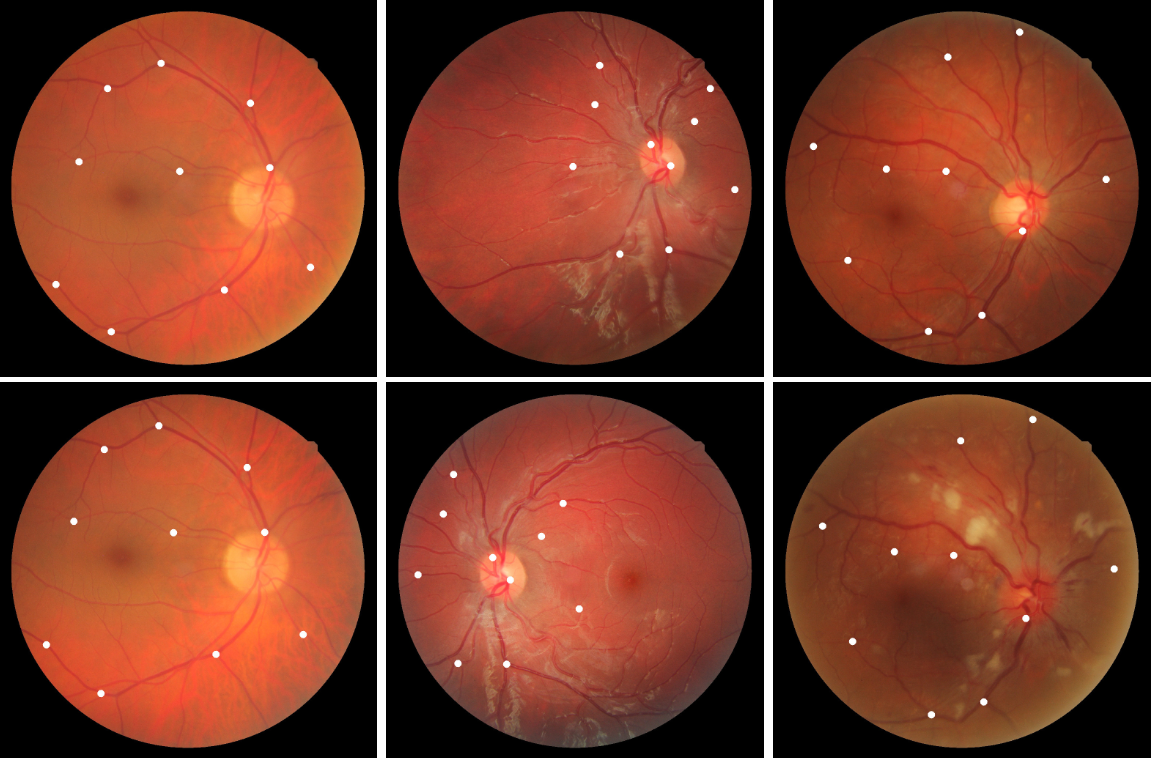
\includegraphics[width=0.95\textwidth]{../imaxes/fire-ej.png}\\
            \small FIRE
        \end{minipage}
        \hspace{0.1\textwidth}
        \begin{minipage}{0.4\textwidth}
            \centering
            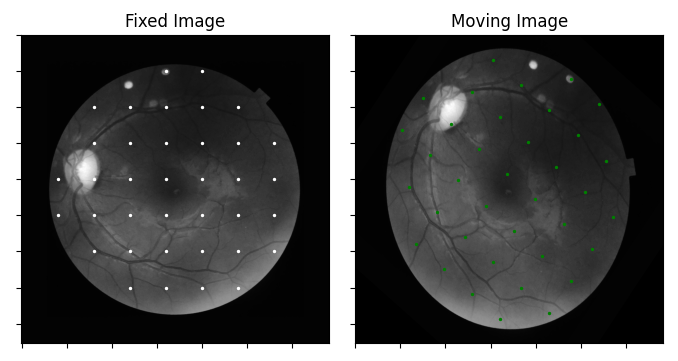
\includegraphics[width=0.95\textwidth]{../imaxes/rfmid_ej.png}\\
            \small RFMID
        \end{minipage}
        
        % \vspace{0.2cm}
        % \small{Exemplos do dataset FIRE e RFMID.}
    \end{center}
    % NOTAS PARA O PRESENTADOR:
    % - Explica a estratexia dos dous datasets. "Para avaliar o noso método de forma completa, utilizamos dous conxuntos de datos moi diferentes."
    % - Describe RFMID: "Primeiro, un dataset sintético que creamos a partir de RFMID. Aquí, nós aplicamos as deformacións, polo que coñecemos a solución exacta. Isto permítenos illar e medir a capacidade pura do modelo para aprender unha transformación xeométrica, sen outras complicacións."
    % - Describe FIRE: "Despois, probamos o modelo no 'mundo real' co dataset FIRE. Estas son imaxes clínicas reais, con todos os seus problemas: diferente iluminación, baixo contraste, enfermidades e, o máis difícil, áreas que non se solapan. Este dataset pon a proba a robustez do noso método."
    % - A lóxica é clara: "Se un modelo funciona en RFMID pero non en FIRE, sabemos que o problema non é a súa capacidade xeométrica, senón a súa fraxilidade ante as variacións de aparencia. Esta estratexia permítenos diagnosticar mellor o comportamento do modelo."
\end{frame}

\begin{frame}
    \frametitle{Métrica de Avaliación}
    \begin{alertblock}{Protocolo de Avaliación}
        Usamos o protocolo estándar de FIRE: unha gráfica que mostra a \textbf{porcentaxe de rexistros exitosos} para un limiar de erro crecente. \textbf{Máis alto e á esquerda é mellor}.
    \end{alertblock}

    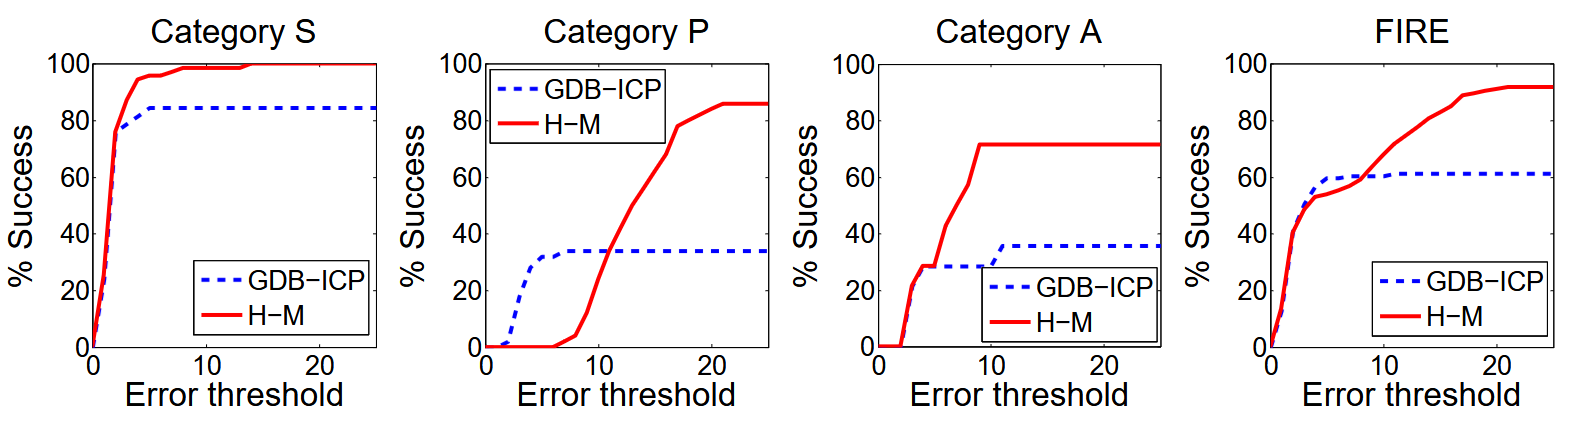
\includegraphics[width=0.95\textwidth]{../imaxes/fire_aval.png}



    % NOTAS PARA O PRESENTADOR:
    % - Explica a métrica de forma sinxela: "Para comparar resultados, usamos a métrica estándar de FIRE. É unha gráfica onde o ideal é estar o máis arriba e á esquerda posible. Isto significa que conseguimos moitos rexistros correctos con moi pouco erro."
\end{frame}


\begin{frame}
    \frametitle{Análise Cualitativa}
    
    \begin{block}{Análise Visual}
        A avaliación visual é crucial para entender \textit{como} e \textit{por que} o método funciona ou falla.
    \end{block}

            \centering
            \textbf{Rexistro Exitoso (RFMiD, ReLU)}
            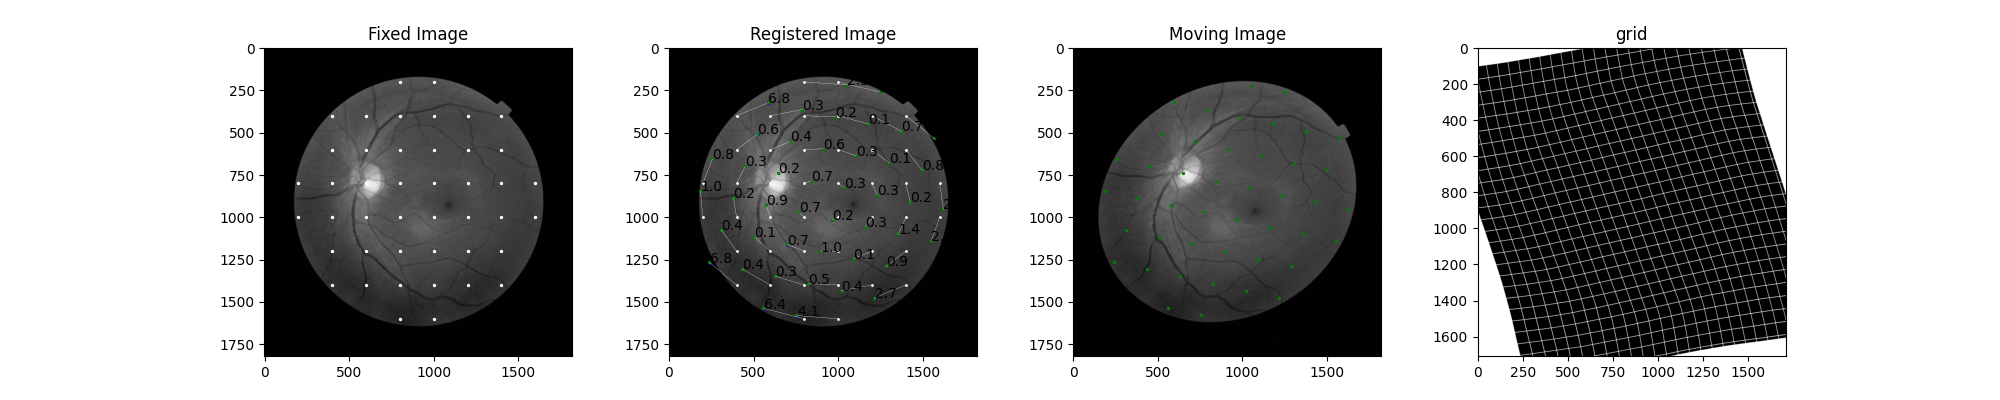
\includegraphics[width=\textwidth]{../imaxes/reg_examples/RFMID_MLP_buena.png}
            \small{A grella de deformación é suave e os puntos de control (azul) axústanse correctamente.}

    
    % NOTAS PARA O PRESENTADOR:
    % - "Pero os números non o son todo. Vexamos que pasa realmente."
    % - "Á esquerda, un caso de éxito. A grella de abaixo é suave, coma se estirásemos unha goma. Os puntos de control azuis (os que move a rede) caen sobre os brancos (os obxectivo)."
    % - "Á dereita, un fracaso. A rede, intentando aliñar, 'rompe' a imaxe. A grella está pregada sobre si mesma, algo fisicamente imposible. Isto é o que a regularización intenta evitar."
\end{frame}


% \begin{frame}
%     \frametitle{Resultados Cuantitativos: ReLU vs. SIREN}
    
%     \begin{block}{Achado Principal: O rendemento depende da complexidade do problema}
%         Non hai un gañador absoluto. A arquitectura óptima depende da natureza da transformación a aprender.
%     \end{block}
    
%     \begin{columns}
%         \begin{column}{0.5\textwidth}
%             \centering
%             \begin{tabular}{lcc}
%                 \toprule
%                 \textbf{Método} & \textbf{Dataset} & \textbf{Dist. Media (px) $\downarrow$} \\
%                 \midrule
%                 MLP-ReLU & RFMID (Sinxelo) & \textbf{Moi Baixo} \\
%                 MLP-SIREN & RFMID (Sinxelo) & Lixeiramente Maior \\
%                 \midrule
%                 MLP-ReLU & FIRE (Complexo) & Alto \\
%                 \rowcolor{ficblue!20}
%                 \textbf{MLP-SIREN} & \textbf{FIRE (Complexo)} & \textbf{Lixeiramente Mellor} \\
%                 \bottomrule
%             \end{tabular}
%             \small{table}{Resumo simplificado dos resultados. Datos de.[1]}
            
%             \vspace{0.5cm}
%             \textbf{Outros achados clave}:
%             \begin{itemize}
%                 \item O \textbf{tamaño do lote (\textit{tamaño de lote})} é un dos parámetros máis críticos. Lotes grandes ($>10000$) son esenciais.[1]
%                 \item O rexistro falla cando a \textbf{superposición} entre imaxes é baixa ($<75\%$, categoría P de FIRE).[1]
%             \end{itemize}
%         \end{column}
        
%         \begin{column}{0.5\textwidth}
%             \centering
%         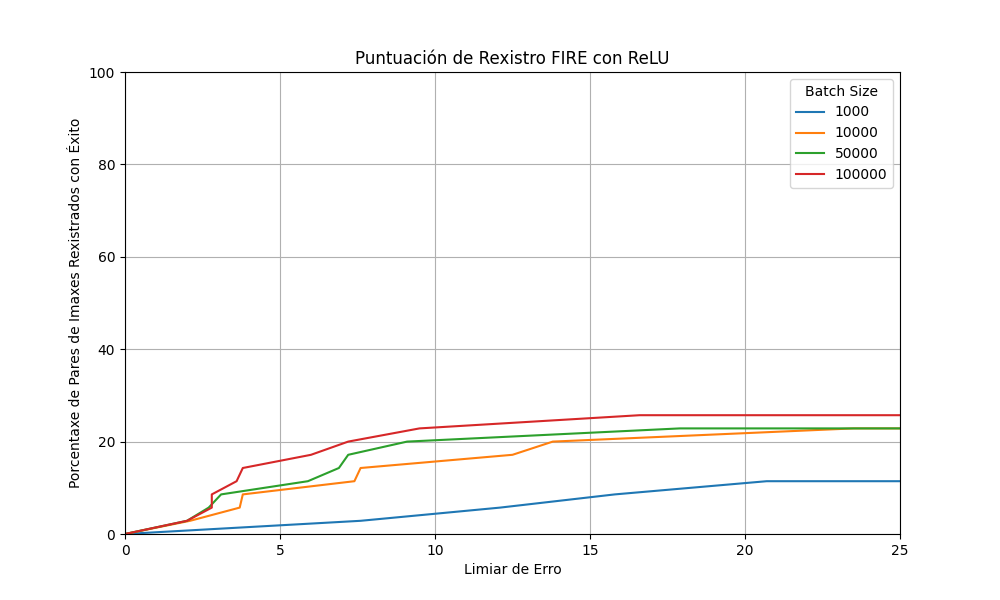
\includegraphics[width=\textwidth]{../imaxes/batchsize/fire_registration_scores_bs_relu_S.png}
%                 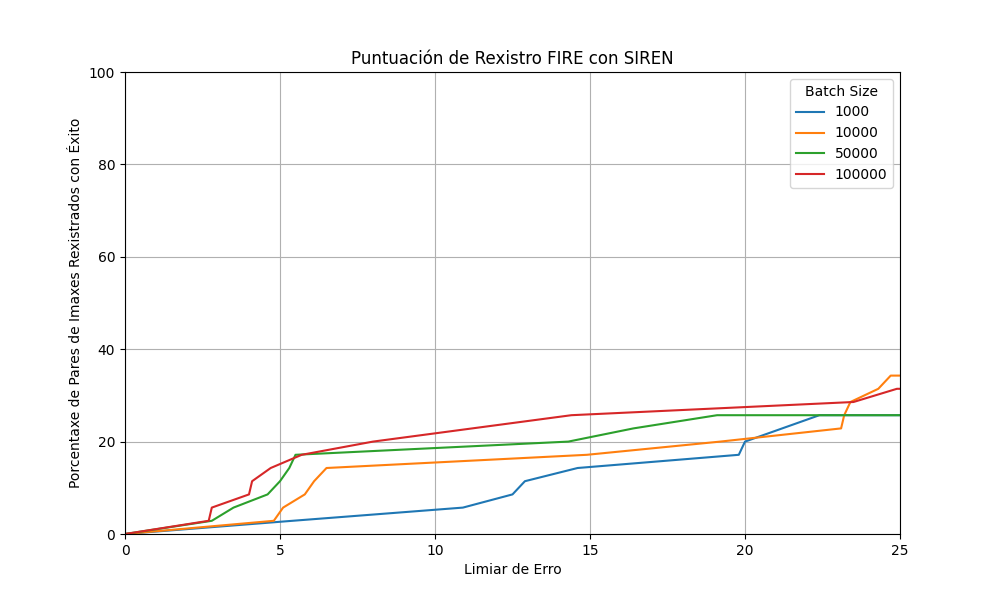
\includegraphics[width=\textwidth]{../imaxes/batchsize/fire_registration_scores_bs_siren_S.png}    
%         \small{figure}{Comparativa de rendemento en FIRE (Cat. S). Adaptado de.[1]}
%         \end{column}
%     \end{columns}
    
%     % NOTAS PARA O PRESENTADOR:
%     % - Este é o slide de resultados máis importante. Sexa claro e directo.
%     % - Comeza coa táboa: "Os nosos experimentos revelaron un resultado interesante e cheo de matices. Non hai unha arquitectura que sexa sempre mellor."
%     % - Explica a primeira parte (RFMID): "No noso dataset sintético, con transformacións sinxelas e globais, a rede con ReLU funciona mellor. A súa natureza máis simple é unha vantaxe para problemas simples."
%     % - Explica a segunda parte (FIRE): "Pero, cando pasamos ao dataset real FIRE, con deformacións locais e complexas, SIREN toma a dianteira, aínda que por unha marxe pequena. A súa capacidade para modelar detalles finos, como prediciamos, dálle unha vantaxe."
%     % - Mostra a gráfica: "Esta gráfica do dataset FIRE confirma visualmente que SIREN (en laranxa) consegue un rendemento lixeiramente superior a ReLU (en azul)."
%     % - Menciona os outros factores críticos: "Ademais da arquitectura, descubrimos que dous factores son absolutamente clave: usar un tamaño de lote moi grande para darlle á rede suficiente información en cada paso, e que o método ten dificultades cando as imaxes se solapan pouco."
%     % - Conclusión da diapositiva: "A lección principal é que a elección da arquitectura debe coincidir coa complexidade do problema. Non hai unha solución única."
% \end{frame}

% \begin{frame}
%     \frametitle{Análise Cualitativa: Éxitos e Fracasos}
    
%     \begin{block}{Unha imaxe vale máis que mil números}
%         A avaliación visual é crucial para entender \textit{como} e \textit{por que} o método funciona ou falla.
%     \end{block}
    
%     \begin{columns}
%         \begin{column}{0.5\textwidth}
%             \centering
%             \textbf{Rexistro Exitoso (RFMiD, ReLU)}
%         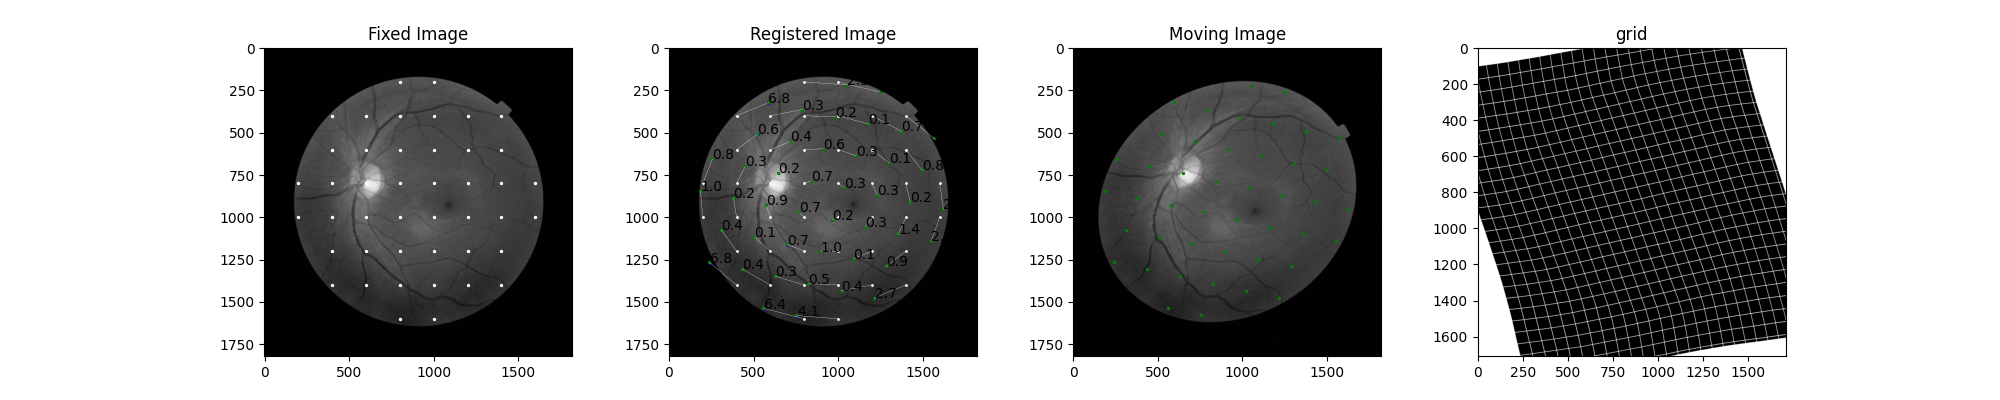
\includegraphics[width=\textwidth]{../imaxes/reg_examples/RFMID_MLP_buena.png}
%         \end{column}
        
%         \begin{column}{0.5\textwidth}
%             \centering
%             \textbf{Rexistro Fallido (RFMiD, ReLU)}
%         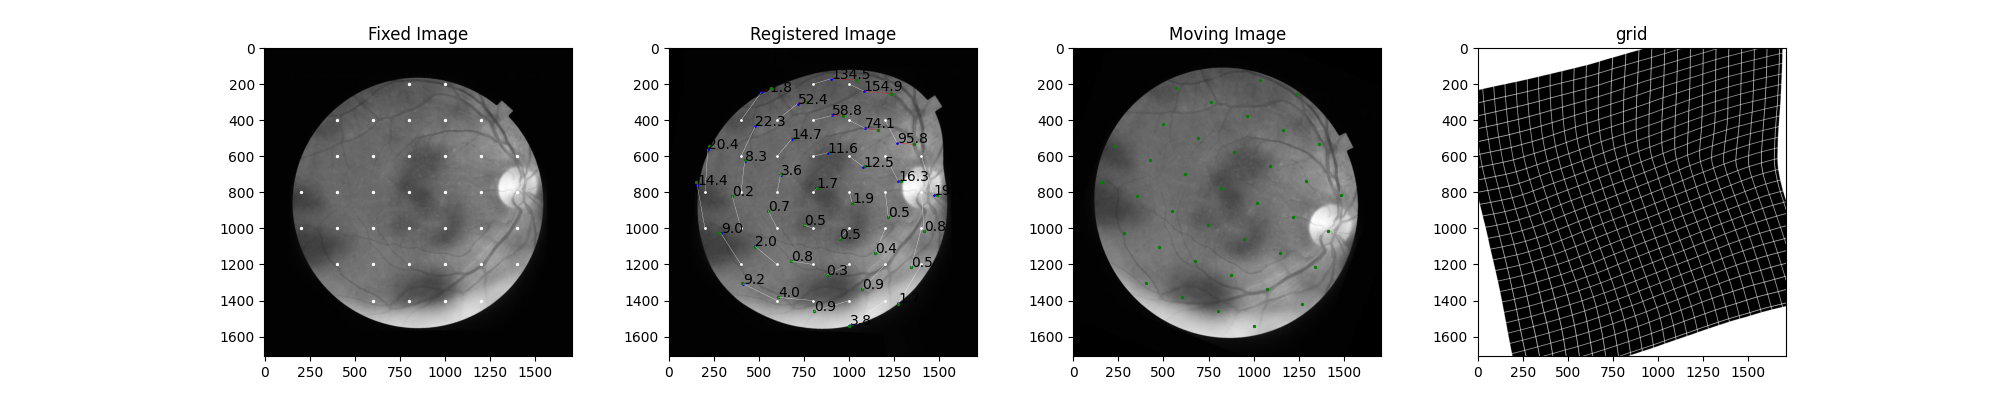
\includegraphics[width=\textwidth]{../imaxes/reg_examples/RFMID_MLP_mala.png}
%         \end{column}
%     \end{columns}
%     % NOTAS PARA O PRESENTADOR:
%     % - "Os números son importantes, pero as imaxes permítennos ver o que realmente está a pasar."
%     % - Mostra o exemplo de éxito: "Á esquerda temos un rexistro exitoso. Se nos fixamos na imaxe de 'checkerboard', vemos como os vasos sanguíneos flúen sen interrupcións entre os cadrados. Isto indica un aliñamento moi preciso. A grella de deformación de abaixo é suave e fisicamente plausible."
%     % - Mostra o exemplo de fracaso: "Á dereita, un caso de fracaso. Os vasos están claramente desalineados e 'rotos' no checkerboard. O máis interesante é a grella de deformación. Vemos como se prega sobre si mesma, creando unha transformación que é imposible no mundo físico. Isto é un sinal claro de que a rede, nun intento de aliñar as imaxes, atopou unha solución matematicamente válida pero incorrecta."
%     % - Conclúe a análise: "Esta análise visual é fundamental. Non só confirma os nosos resultados cuantitativos, senón que nos axuda a diagnosticar os modos de fallo do modelo, o que nos dá pistas sobre como melloralo no futuro."
% \end{frame}


% ------------------- SECCIÓN 4: EXPERIMENTOS E RESULTADOS ---------------------- %
\section{Experimentos e Resultados}

% \begin{frame}
%     \frametitle{Visión Xeral dos Experimentos}
    
%     \begin{block}{Obxectivo Experimental}
%         Avaliar sistematicamente os factores que inflúen no rendemento do rexistro con representacións implícitas (IDIR) para imaxes de retina.
%     \end{block}
    
%     \begin{itemize}
%         \item \textbf{Comparación principal}: Función de activación \textbf{ReLU} vs. \textbf{SIREN}.
%         \item \textbf{Parámetros investigados}:
%         \begin{itemize}
%             \item Función de perda (similitude).
%             \item Resolución da imaxe.
%             \item Peso da regularización.
%             \item Tamaño do lote (\textit{tamaño de lote}).
%         \end{itemize}
%         \item \textbf{Estratexias exploradas}:
%         \begin{itemize}
%             \item Mostraxe de puntos (aleatoria, ponderada, etc.).
%             \item Inicialización dos pesos da rede.
%             \item Axuste dinámico do tamaño do lote.
%         \end{itemize}
%     \end{itemize}
    
%     % NOTAS PARA O PRESENTADOR:
%     % - "Para entender como funciona o noso método, fixemos unha serie de experimentos."
%     % - "O principal era comparar ReLU con SIREN, pero tamén analizamos como afectan a función de perda, a resolución, a regularización e o tamaño do lote."
%     % - "Ademais, probamos algunhas estratexias máis avanzadas como a mostraxe intelixente e diferentes formas de inicializar a rede."
% \end{frame}

\begin{frame}
    \frametitle{Experimentos: Función de Perda}
    
    \begin{block}{Motivación}
        Atopar a métrica de similitude máis robusta para as imaxes de retina.
    \end{block}
    
    \begin{center}
        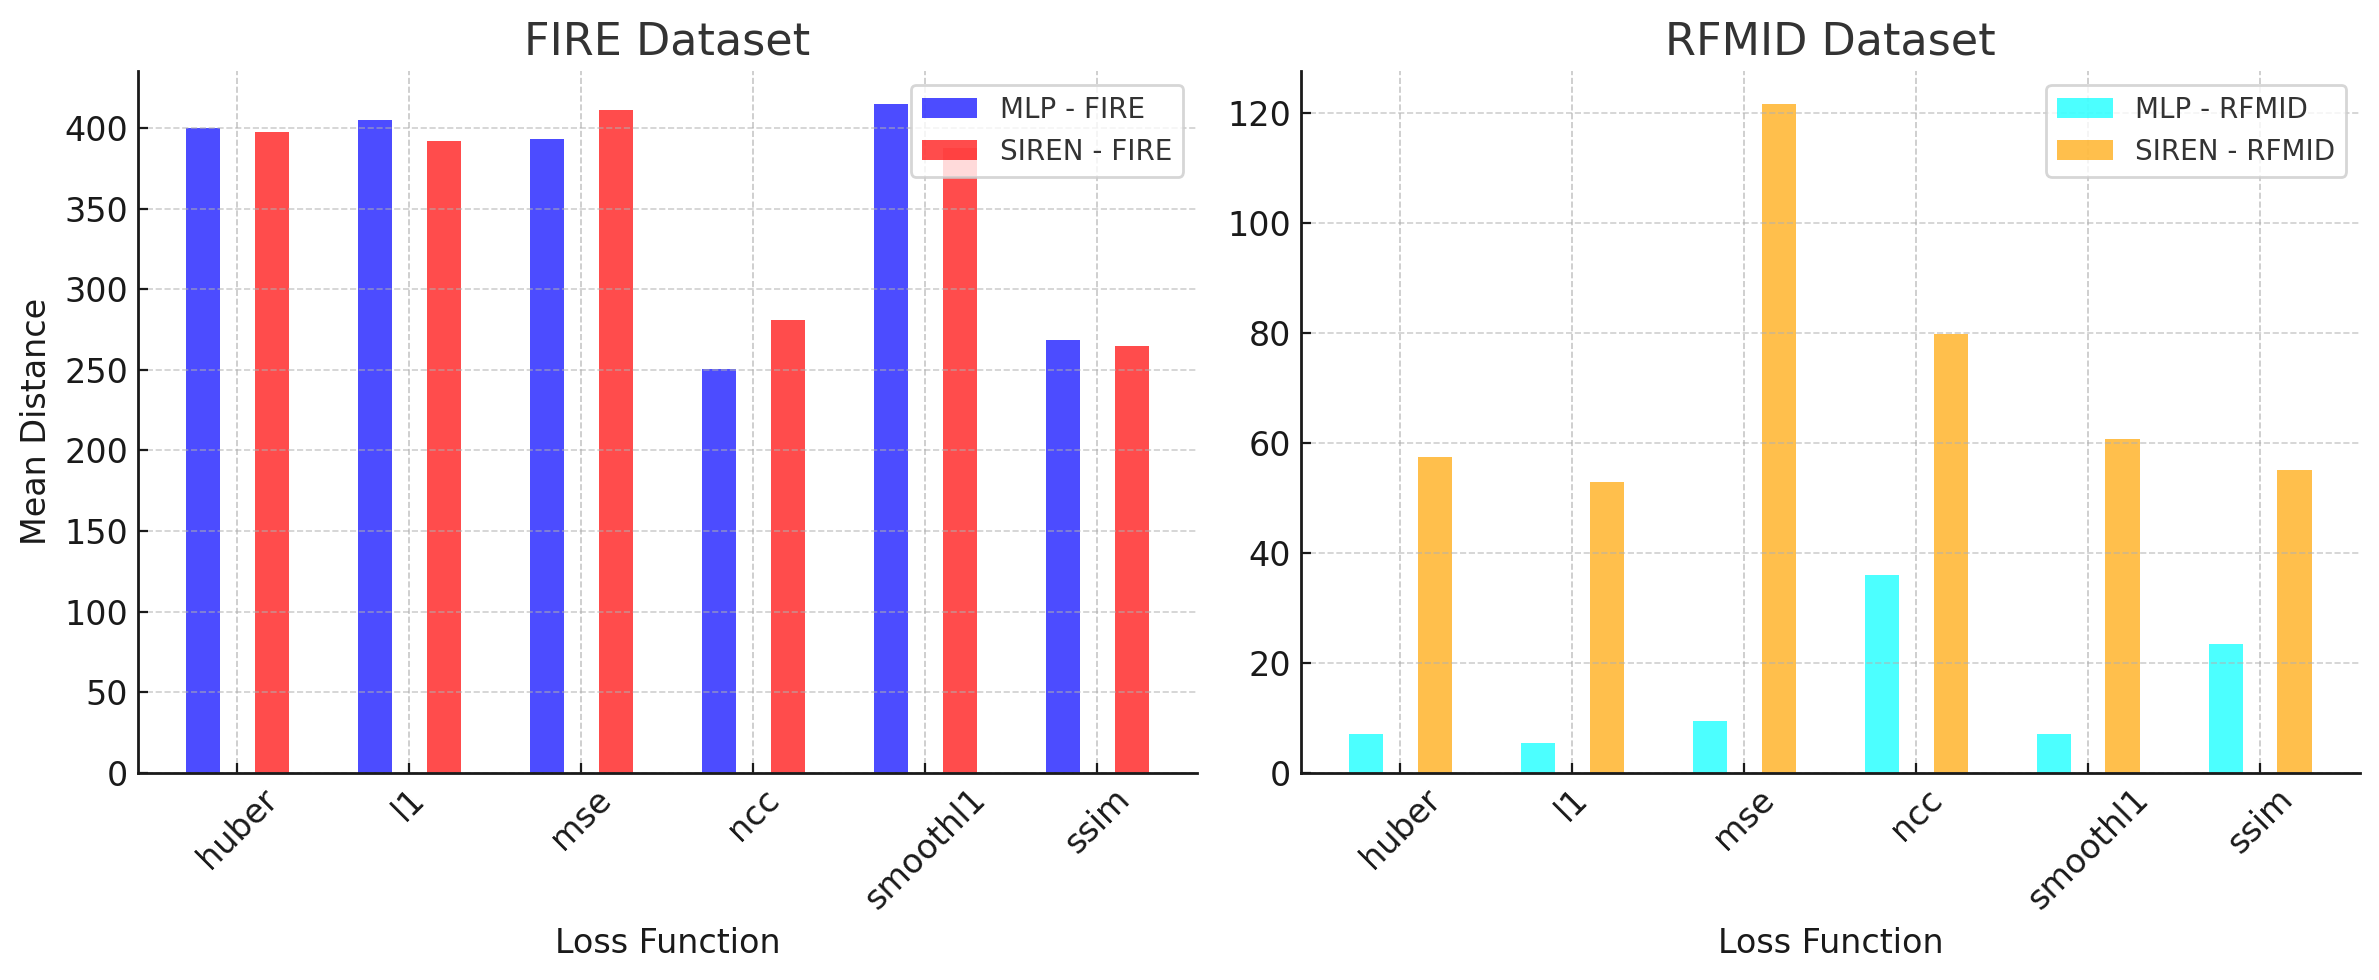
\includegraphics[width=0.9\textwidth]{../imaxes/losstype.png}
    \end{center}
    
    % NOTAS PARA O PRESENTADOR:
    % - "Comezamos por elixir a mellor forma de medir se dúas imaxes se parecen."
    % - "O gráfico mostra as diferentes métricas probadas."
\end{frame}

\begin{frame}
    \frametitle{Experimento: Función de Perda}
    \begin{alertblock}{Conclusión}
        A métrica ideal depende da natureza dos datos:
        \begin{itemize}
            \item \textbf{FIRE}: Métricas estruturais como \textbf{NCC} funcionan mellor.
            \item \textbf{RFMID}: Métricas baseadas en píxeles como \textbf{L1} ou MSE son superiores.
        \end{itemize}
    \end{alertblock}   
    \begin{center}
        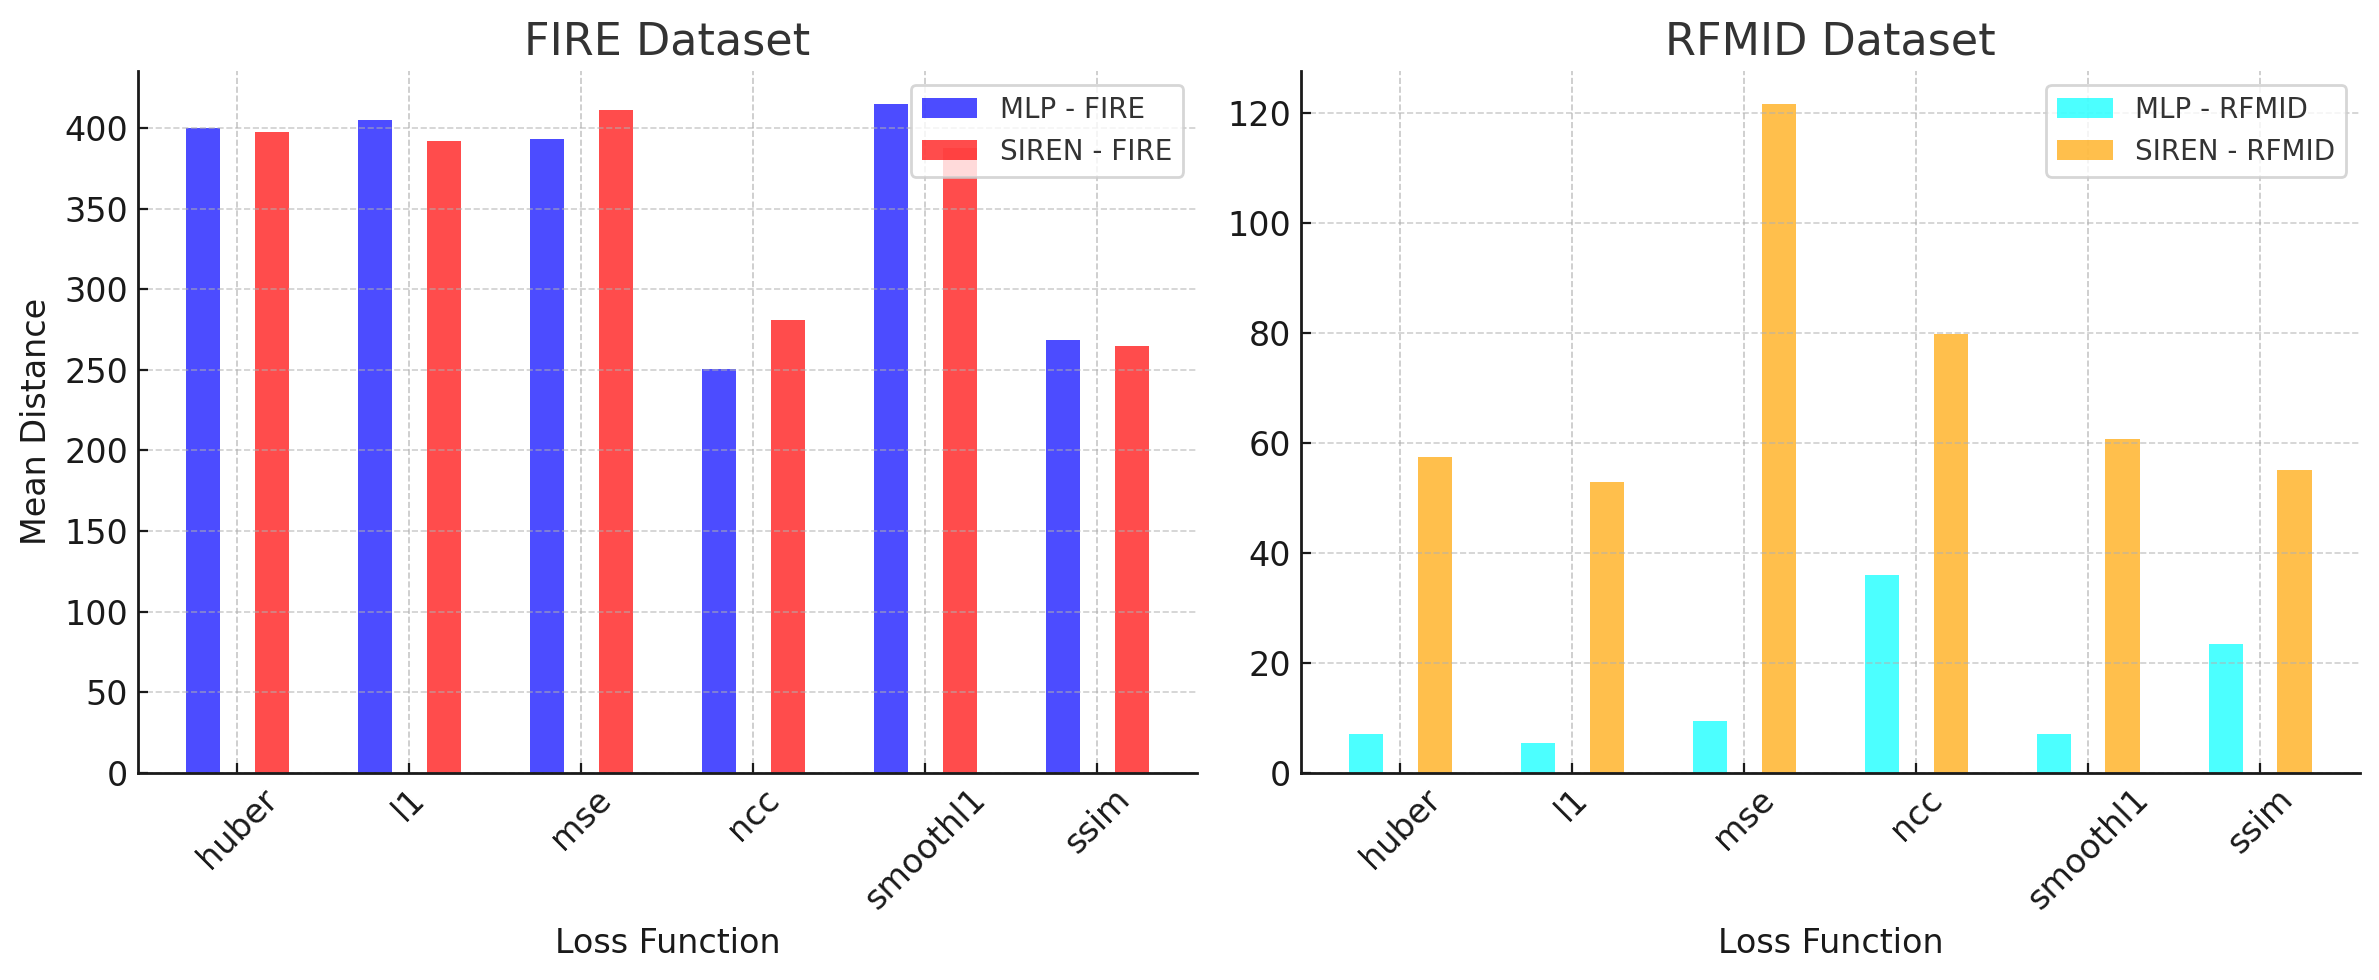
\includegraphics[width=0.9\textwidth]{../imaxes/losstype.png}
    \end{center}
    
    % NOTAS PARA O PRESENTADOR:
    % - "O gráfico mostra claramente que para imaxes reais (FIRE), as métricas que entenden a estrutura, como NCC, son moito mellores (barra azul máis baixa)."
    % - "Pero para imaxes sintéticas sen cambios de iluminación (RFMID), unha simple resta de píxeles como L1 é suficiente."
    % - "Isto dinos que para aplicacións reais, NCC é a opción correcta."
\end{frame}

\begin{frame}
    \frametitle{Experimento: Resolución da Imaxe}

    \begin{block}{Motivación}
        Determinar se usar imaxes de alta resolución (ata 2160x2160px) mellora o resultado ou só aumenta o custo computacional.
    \end{block}

    \centering
    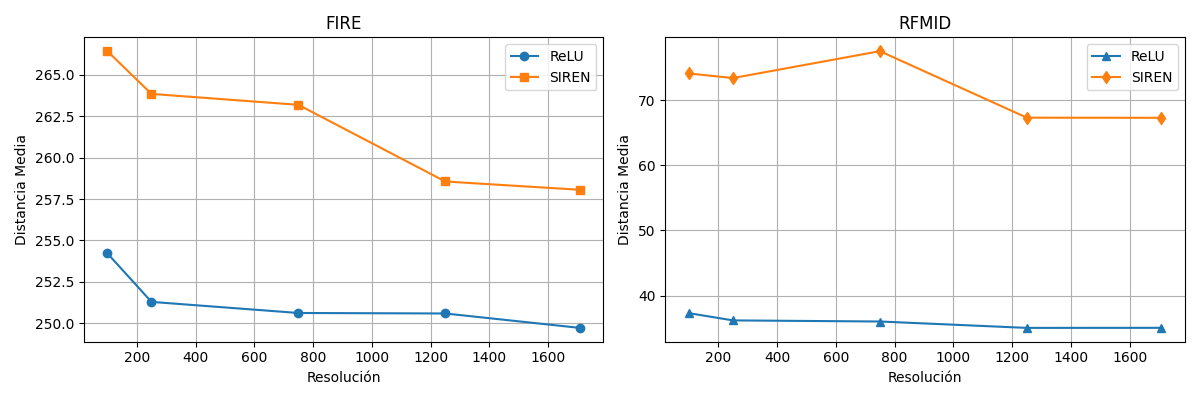
\includegraphics[width=0.9\textwidth]{../imaxes/resolutionchart.png}
    \begin{alertblock}{Conclusión}
        Non se observa unha mellora significativa por enriba de \textbf{1250x1250 píxeles}. Este tamaño ofrece un bo equilibrio.
    \end{alertblock}
    % NOTAS PARA O PRESENTADOR:
    % - "A continuación, preguntámonos: necesitamos toda a resolución da imaxe?"
    % - "Como vemos na gráfica, aínda que hai unha pequena mellora ao aumentar a resolución, esta é marxinal despois dos 1000 píxeles."
\end{frame}

% \begin{frame}
%     \frametitle{Experimento: Resolución da Imaxe}



%     \centering
%     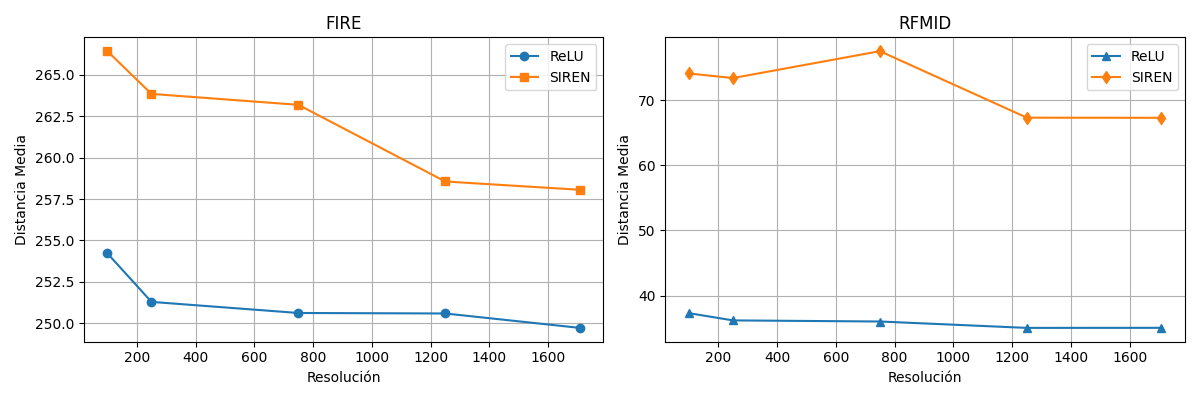
\includegraphics[width=0.9\textwidth]{../imaxes/resolutionchart.png}


%     % NOTAS PARA O PRESENTADOR:
%     % - "Por tanto, para o resto de experimentos, fixamos a resolución en 1000x1000 para ser eficientes sen perder precisión."
% \end{frame}

\begin{frame}
    \frametitle{Experimento: Regularización}
    
    % \begin{block}{Motivación}
    %     Evitar deformacións non realistas (pregamentos, distorsións extremas), especialmente nos modelos SIREN que tenden a solucións de alta frecuencia.
    % \end{block}
    
    \begin{columns}[T]
        \begin{column}{0.35\textwidth}
            \centering
            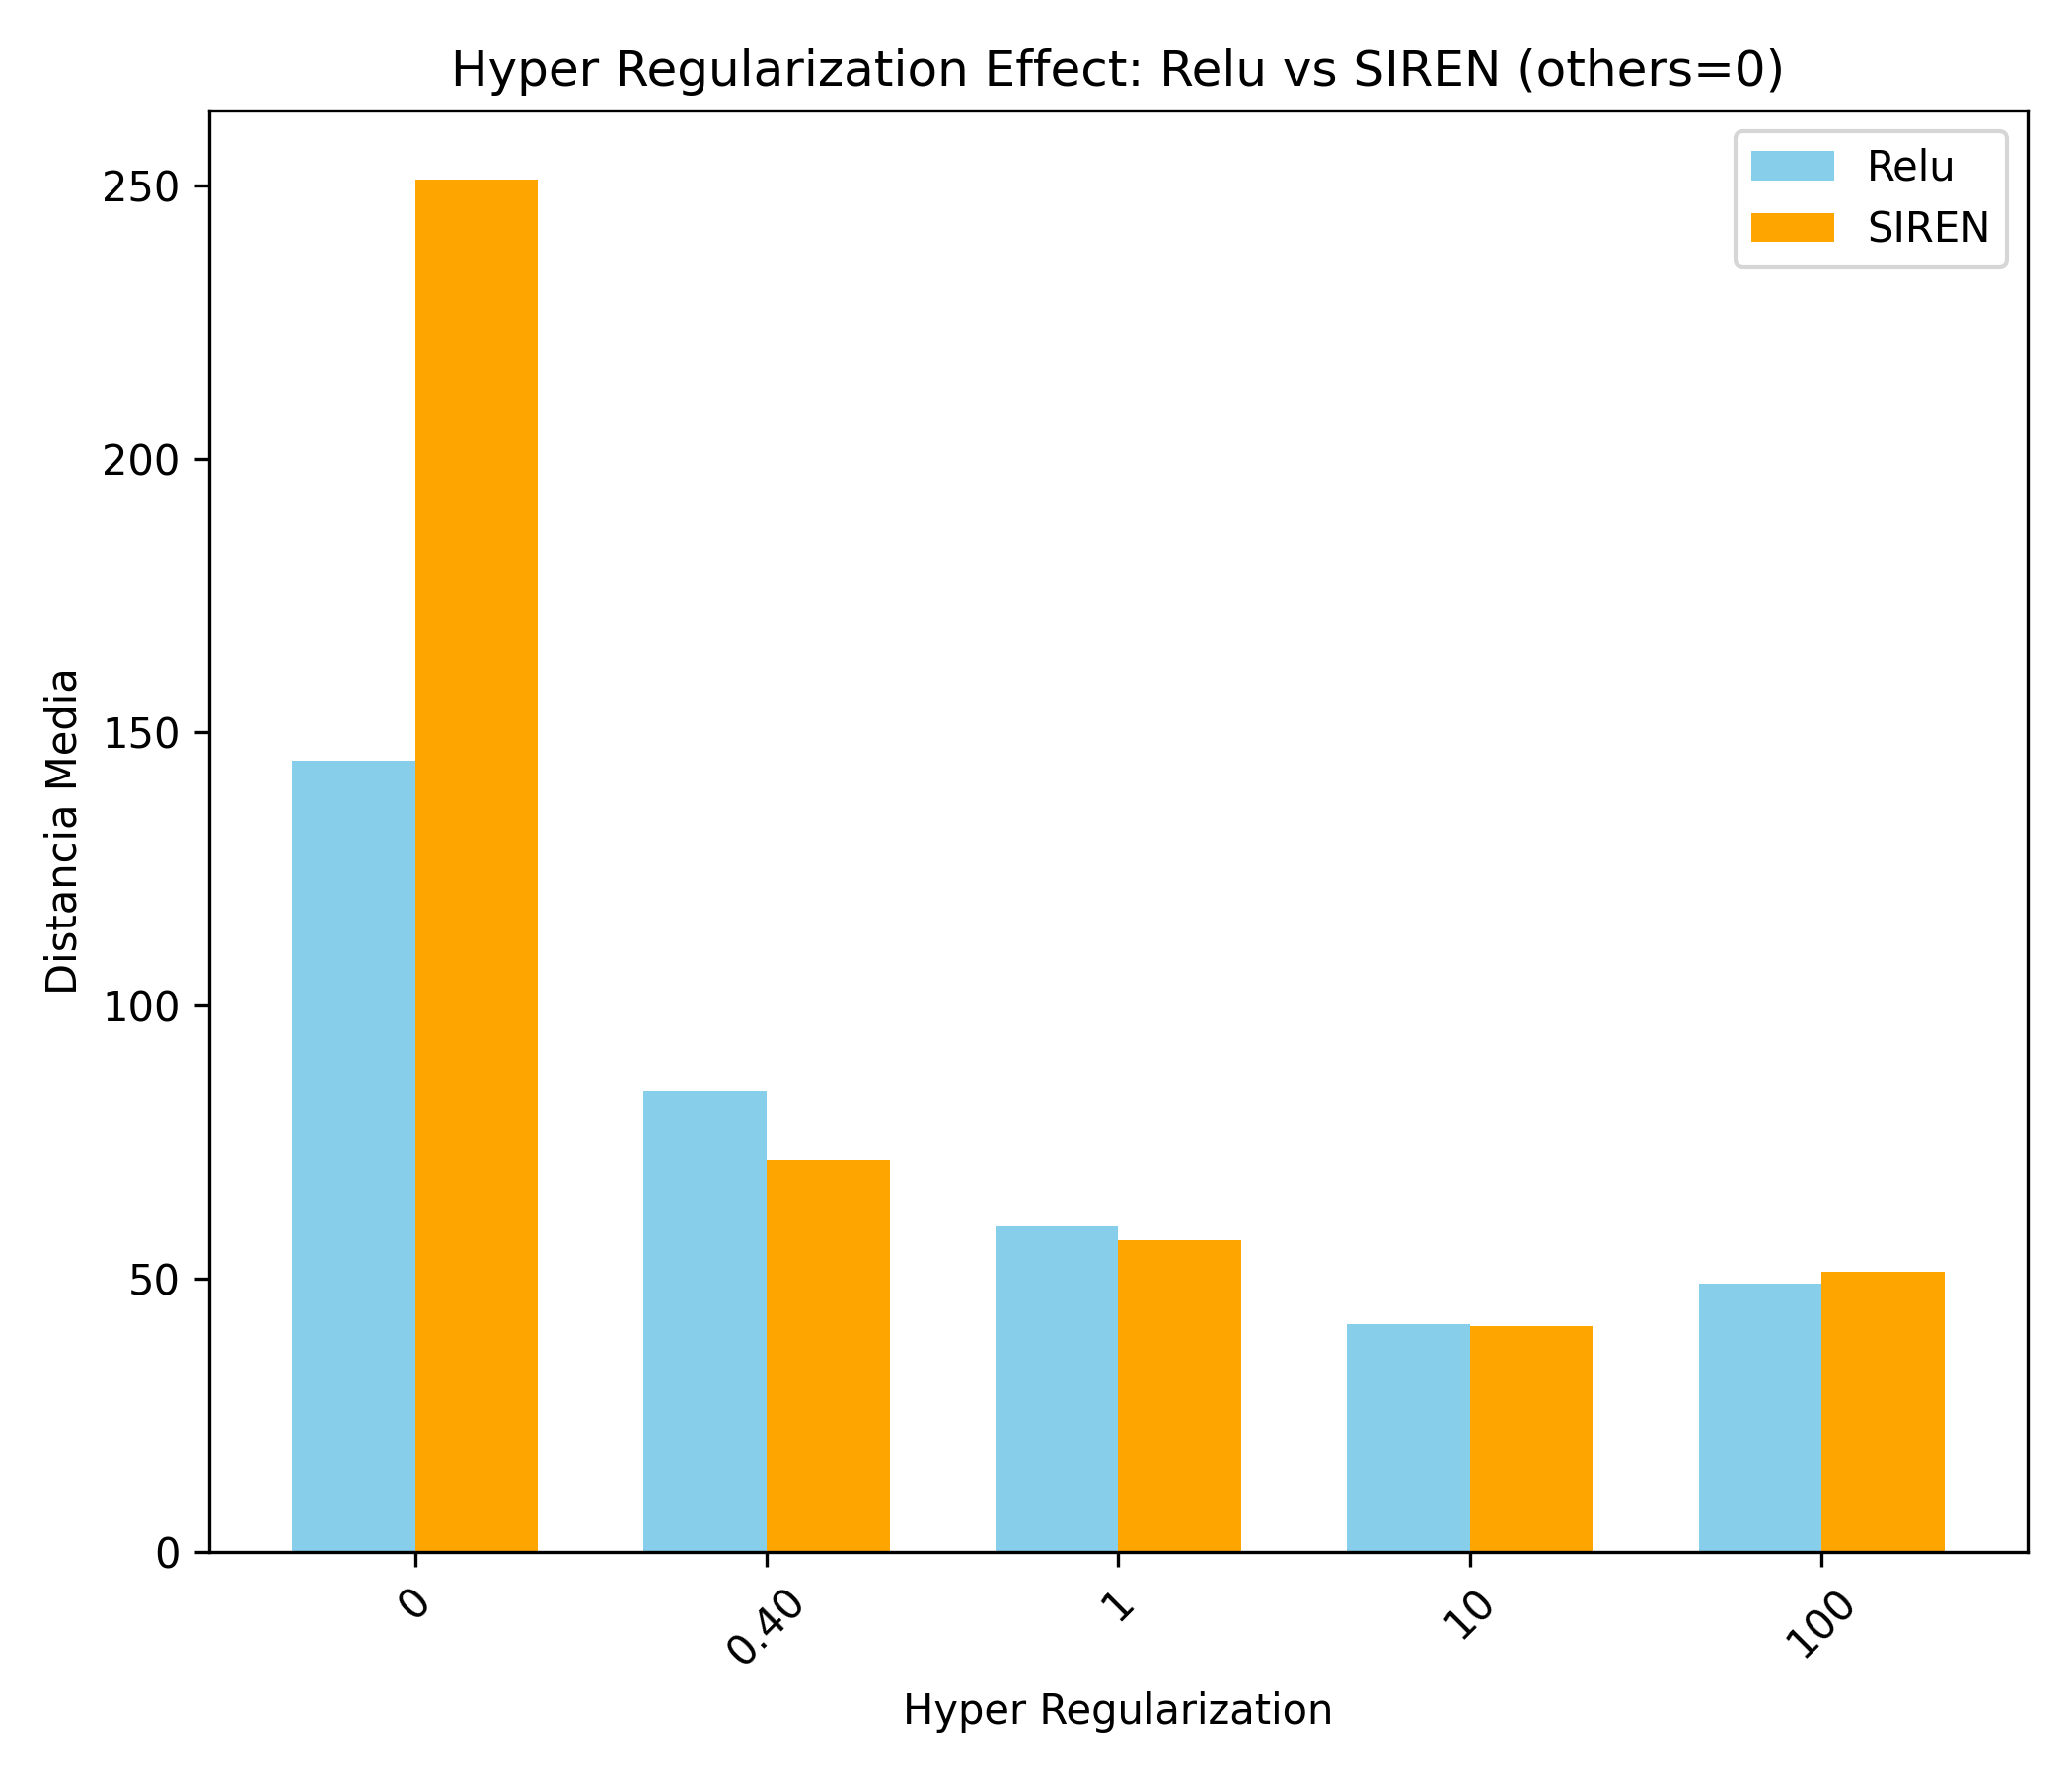
\includegraphics[width=\textwidth]{../imaxes/reg_examples/barplot_hyper_reg_comparison_MLP_vs_SIREN_FIRE.png}
            \small{Regularización hiperelástica en FIRE}
        \end{column}
        \begin{column}{0.35\textwidth}
            \centering
            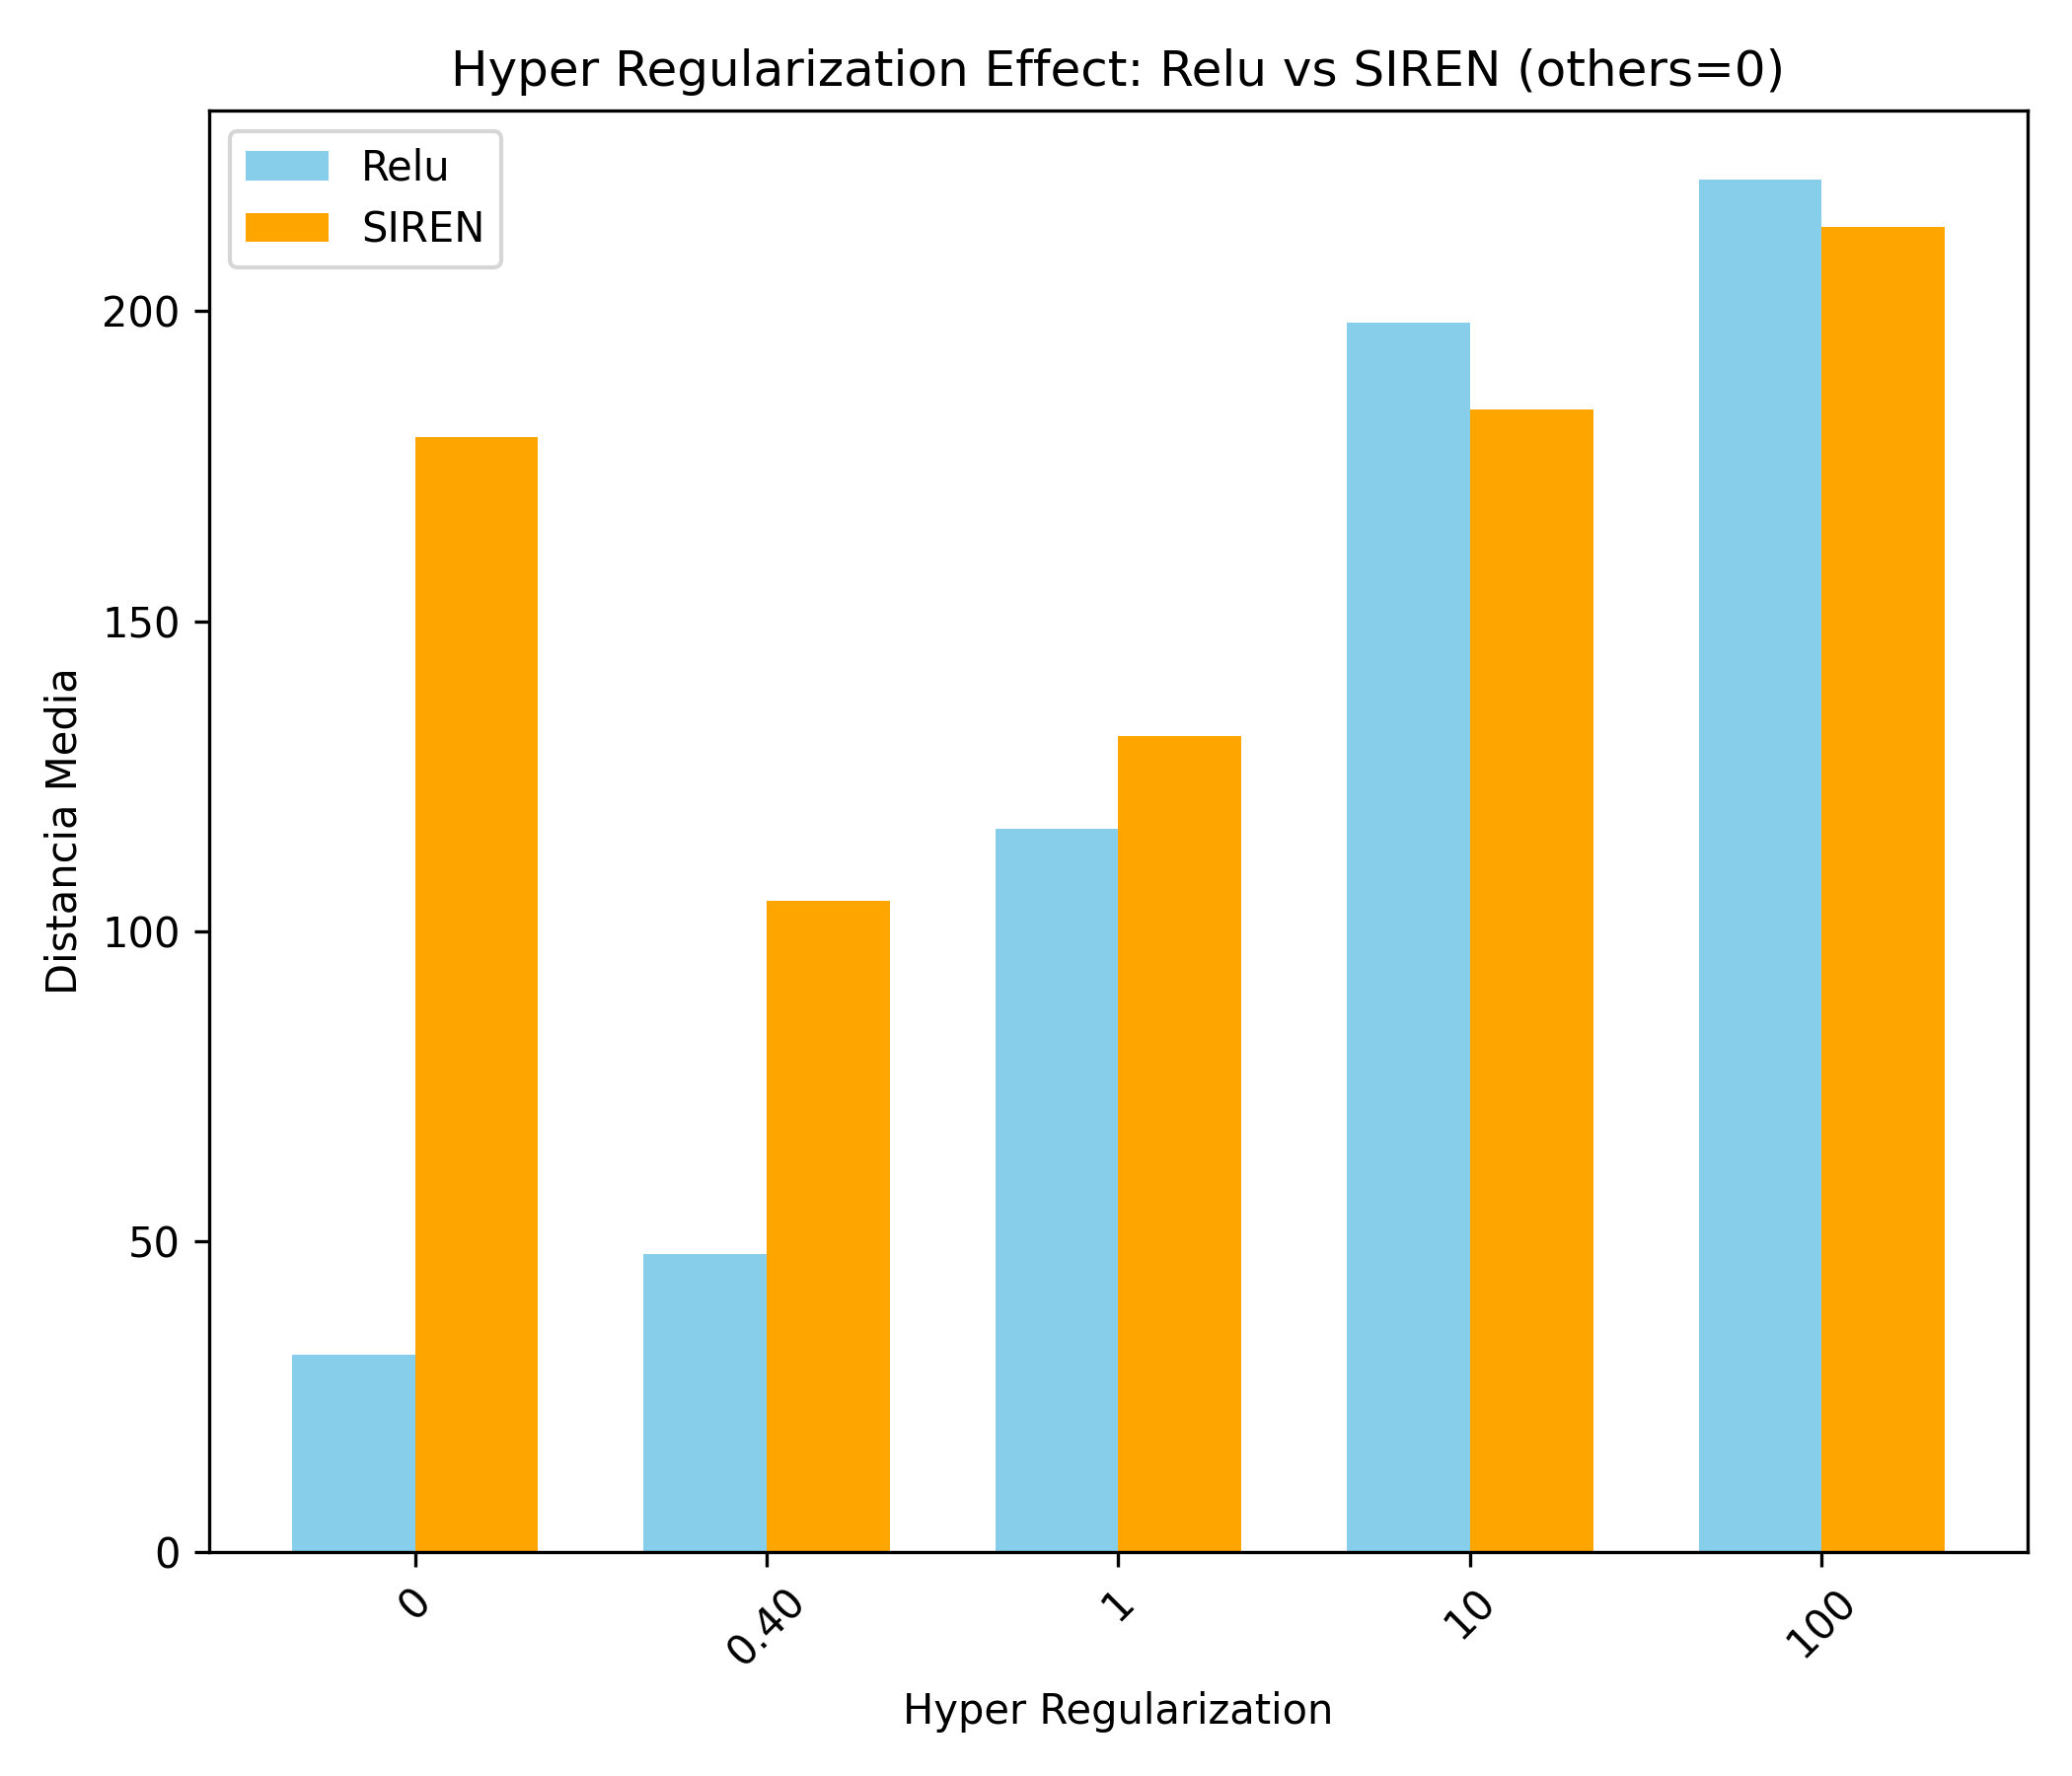
\includegraphics[width=\textwidth]{../imaxes/reg_examples/barplot_hyper_reg_comparison_MLP_vs_SIREN_RFMID.png}
            \small{Regularización hiperelástica en RFMID}
        \end{column}
    \end{columns}
    
    \vspace{0.2cm}
    
    \begin{alertblock}{Conclusión Principal}
        A regularización é \textbf{indispensable} para SIREN. A cantidade óptima depende transformación concreta: deformacións máis complexas (FIRE) benefícianse de maior regularización.
    \end{alertblock}
    
    % NOTAS PARA O PRESENTADOR:
    % - "A regularización é como poñerlle regras físicas á rede."
    % - "Á esquerda, vemos o que pasa sen regras: a rede crea unha deformación imposible, con pregamentos. Á dereita, con demasiadas regras, a deformación é demasiado ríxida e non aliña ben."
    % - "A lección é que necesitamos un equilibrio. E ese equilibrio cambia: problemas máis difíciles necesitan regras máis estritas."
\end{frame}

\begin{frame}
    \frametitle{Experimento: Tamaño do Lote}
    
    % \begin{block}{Motivación}
    %     A análise cualitativa inicial suxeriu que este é un dos parámetros máis críticos para o éxito do adestramento.
    % \end{block}
    
    \begin{columns}[T]
        \begin{column}{0.5\textwidth}
            \centering
            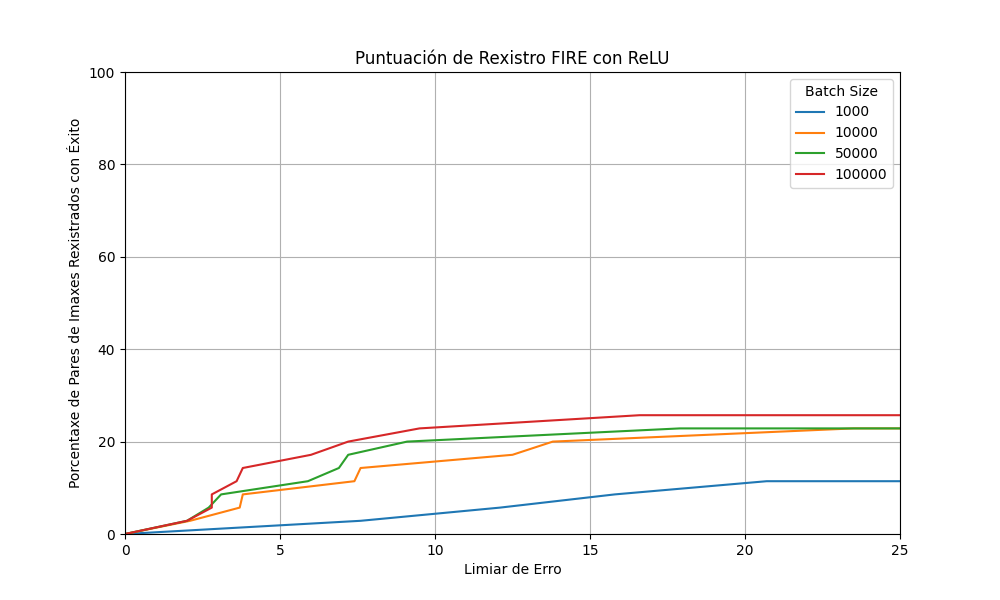
\includegraphics[width=\textwidth]{../imaxes/batchsize/fire_registration_scores_bs_relu_S.png}
                        \small{ReLU (FIRE - Cat. S)}

        \end{column}
        \begin{column}{0.5\textwidth}
            \centering
            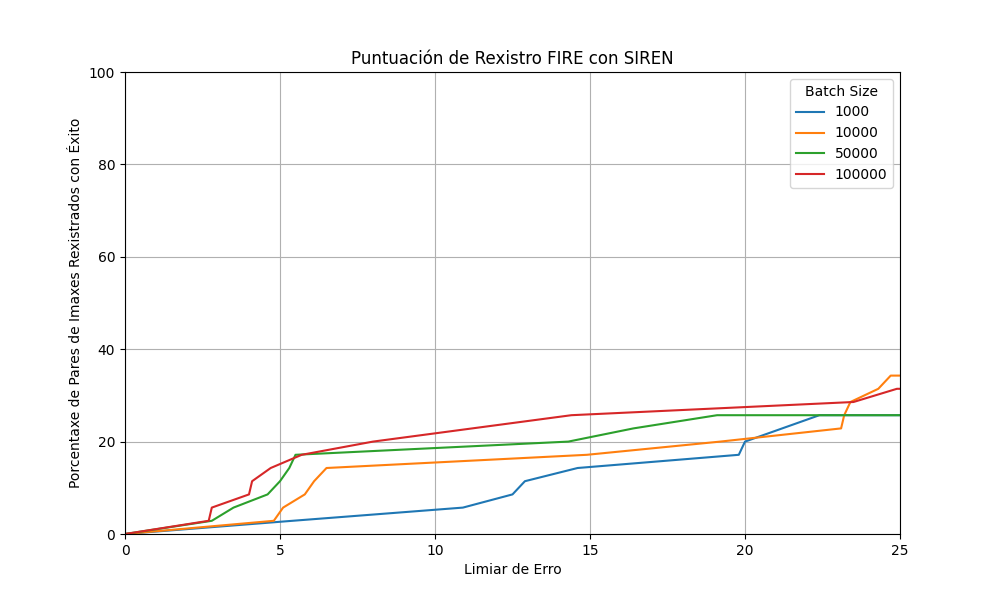
\includegraphics[width=\textwidth]{../imaxes/batchsize/fire_registration_scores_bs_siren_S.png}
                   \small{SIREN (FIRE - Cat. S)}
        \end{column}
    \end{columns}
    
    \begin{alertblock}{Conclusión}
        Un tamaño de lote >10,000 é fundamental para obter bós resultados. Tamaños moi superiores non ofrecen beneficios significativos.
    \end{alertblock}
    
    % NOTAS PARA O PRESENTADOR:
    % - "Este é un dos achados máis importantes do noso traballo."
    % - "Estas gráficas mostran o rendemento no dataset real. A liña laranxa, cun tamaño de lote de 10.000, está moi por riba das outras."
    % - "Isto significa que a rede necesita ver moitos puntos da imaxe en cada paso para entender ben a deformación. Usar lotes pequenos simplemente non funciona."
\end{frame}
% Slide 1: Estratexias de Mostraxe - Visualización e Hipótese
\begin{frame}
    \frametitle{Estratexia Desenvolvida: Mostraxe Intelixente (I)}

    \begin{block}{Hipótese}
        Priorizar rexións con máis información estrutural (vasos sanguíneos, disco óptico) mediante estratexias de mostraxe "intelixentes" podería mellorar o resultado final do rexistro fronte á mostraxe puramente aleatoria.
    \end{block}

    \vspace{0cm}

    \begin{columns}[T]
        \begin{column}{0.3\textwidth}
            \centering
            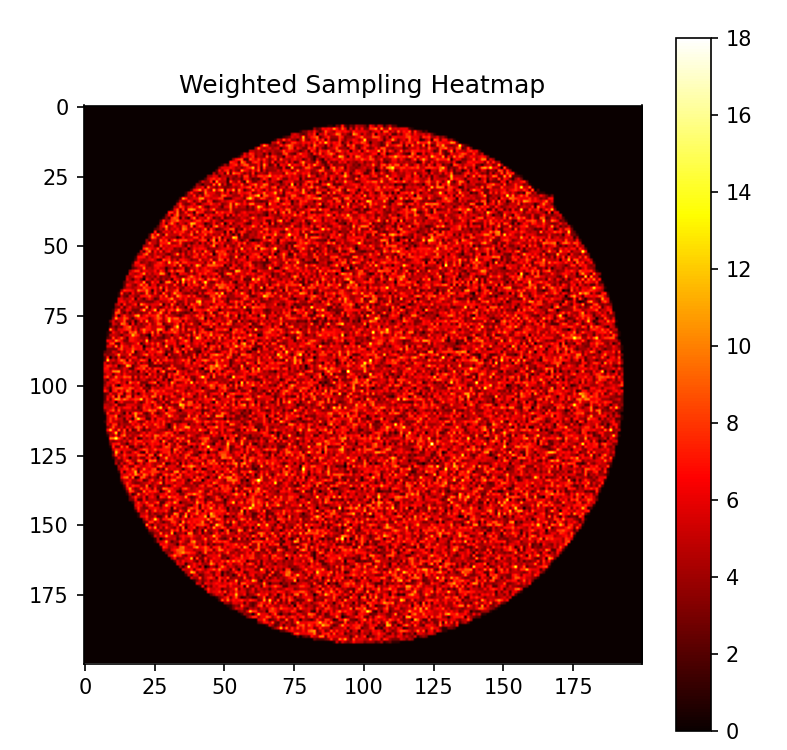
\includegraphics[width=\textwidth]{../imaxes/muestraje/random_sampling_heatmap.png}
            \small{Aleatoria}
        \end{column}
        \begin{column}{0.3\textwidth}
            \centering
            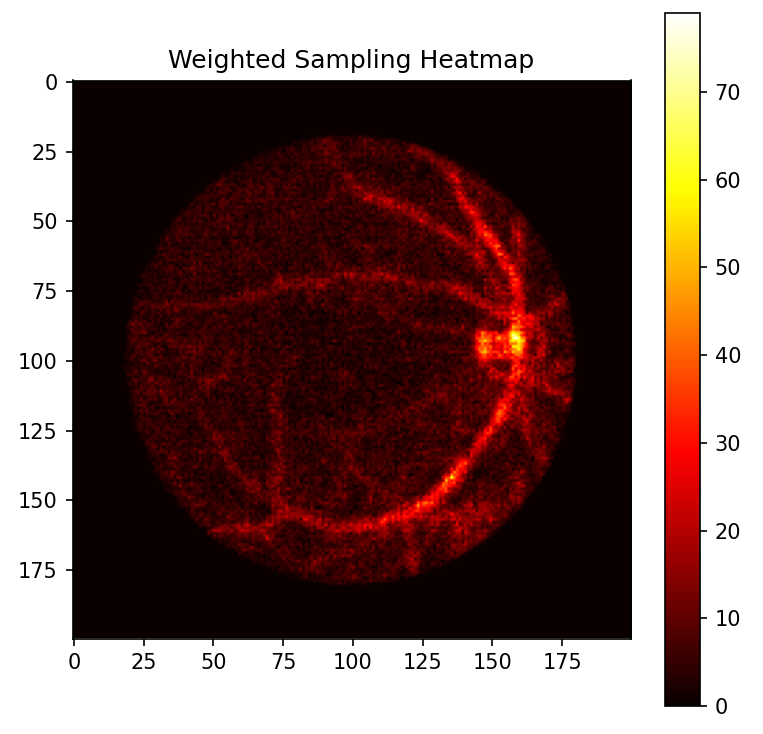
\includegraphics[width=\textwidth]{../imaxes/muestraje/weighted_sampling_heatmap.png}
            \small{Ponderada}
        \end{column}
        \begin{column}{0.3\textwidth}
            \centering            
            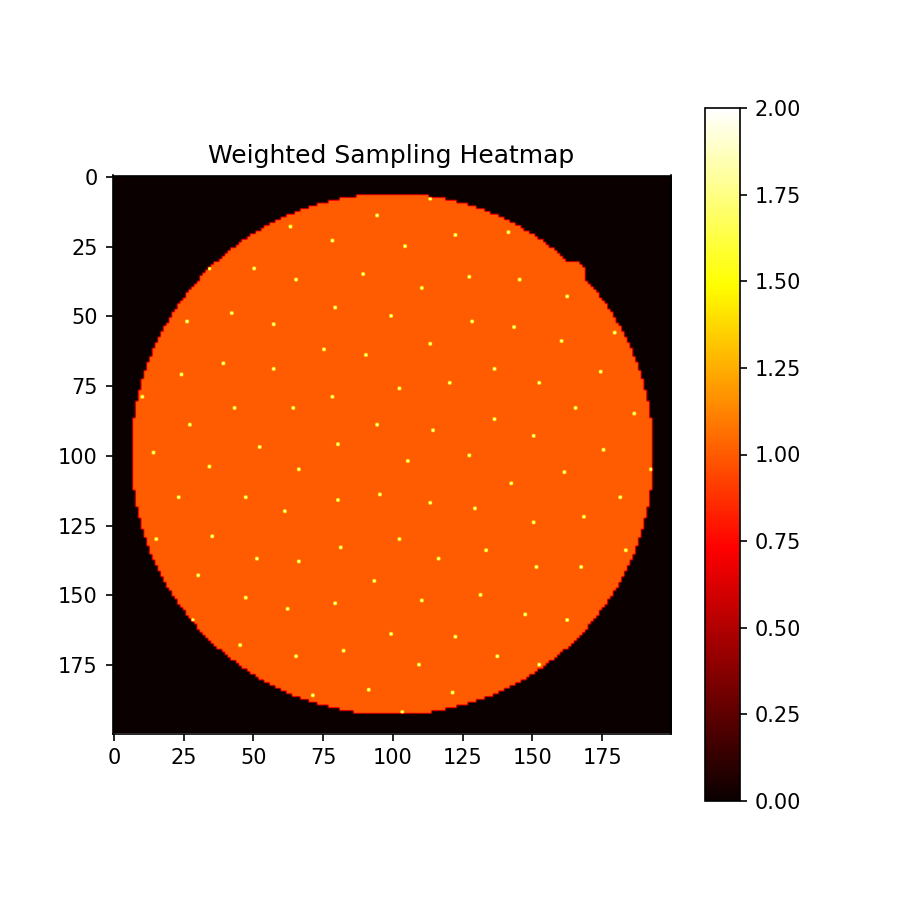
\includegraphics[width=\textwidth]{../imaxes/muestraje/uniform_sampling_heatmap.png}
            \small{Uniforme}
        \end{column}
    \end{columns}
    % \vspace{0.2cm}
    \centering
    % \small{Mapas de calor das diferentes estratexias de mostraxe implementadas.}
\end{frame}
% Slide 2: Estratexias de Mostraxe - Resultados e Conclusión
\begin{frame}
    \frametitle{Estratexia Desenvolvida: Mostraxe Intelixente (II)}

    \begin{columns}[T]
        \begin{column}{0.5\textwidth}
            \centering
            \textbf{ReLU (RFMID)}
            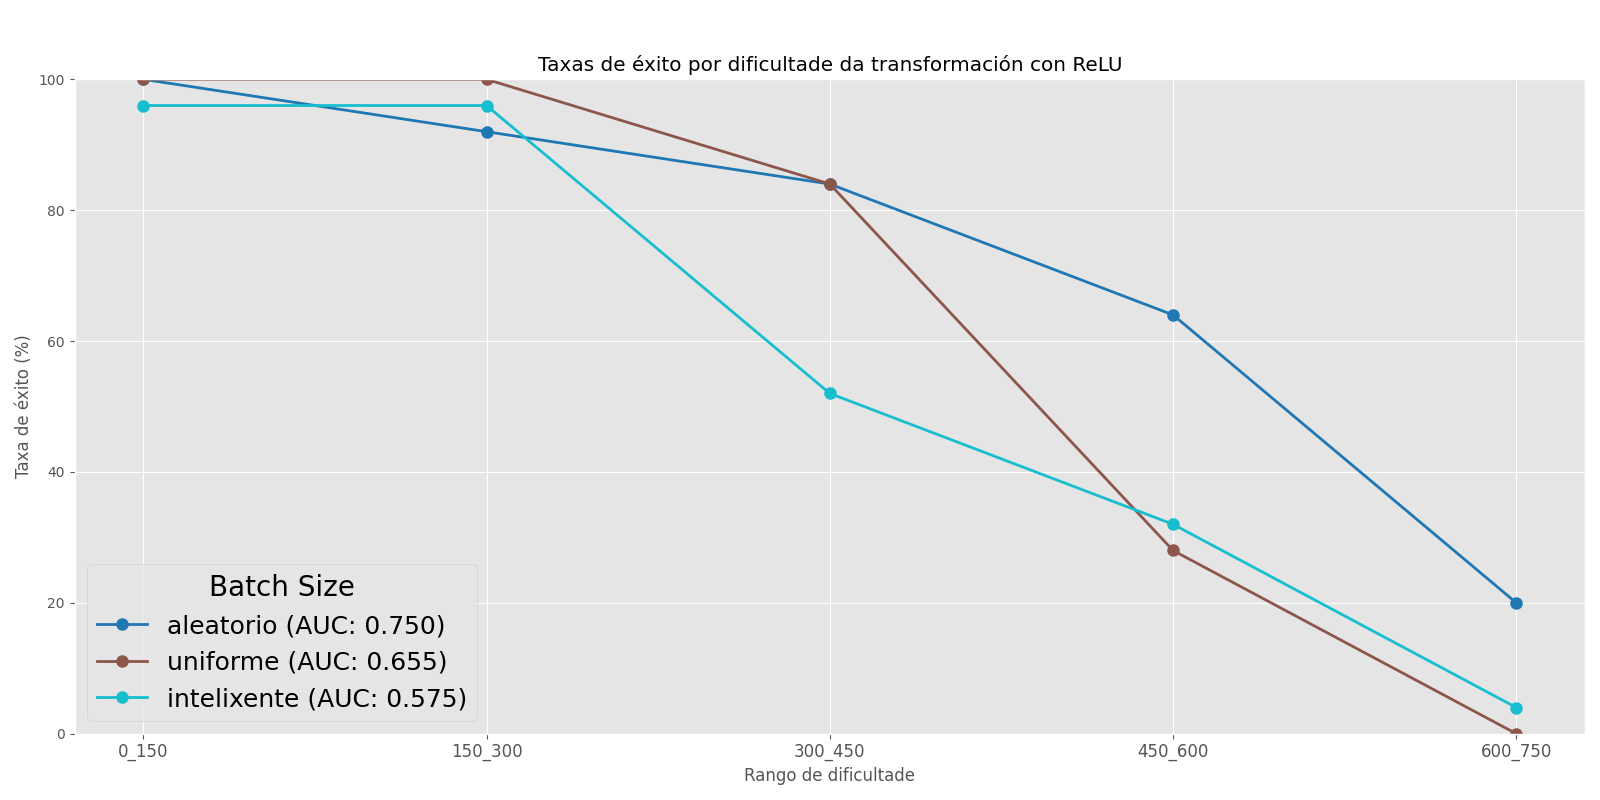
\includegraphics[width=\textwidth]{../imaxes/muestraje/experiment_plot_RFMID_st_relu.png}
        \end{column}
        \begin{column}{0.5\textwidth}
            \centering
            \textbf{SIREN (RFMID)}
            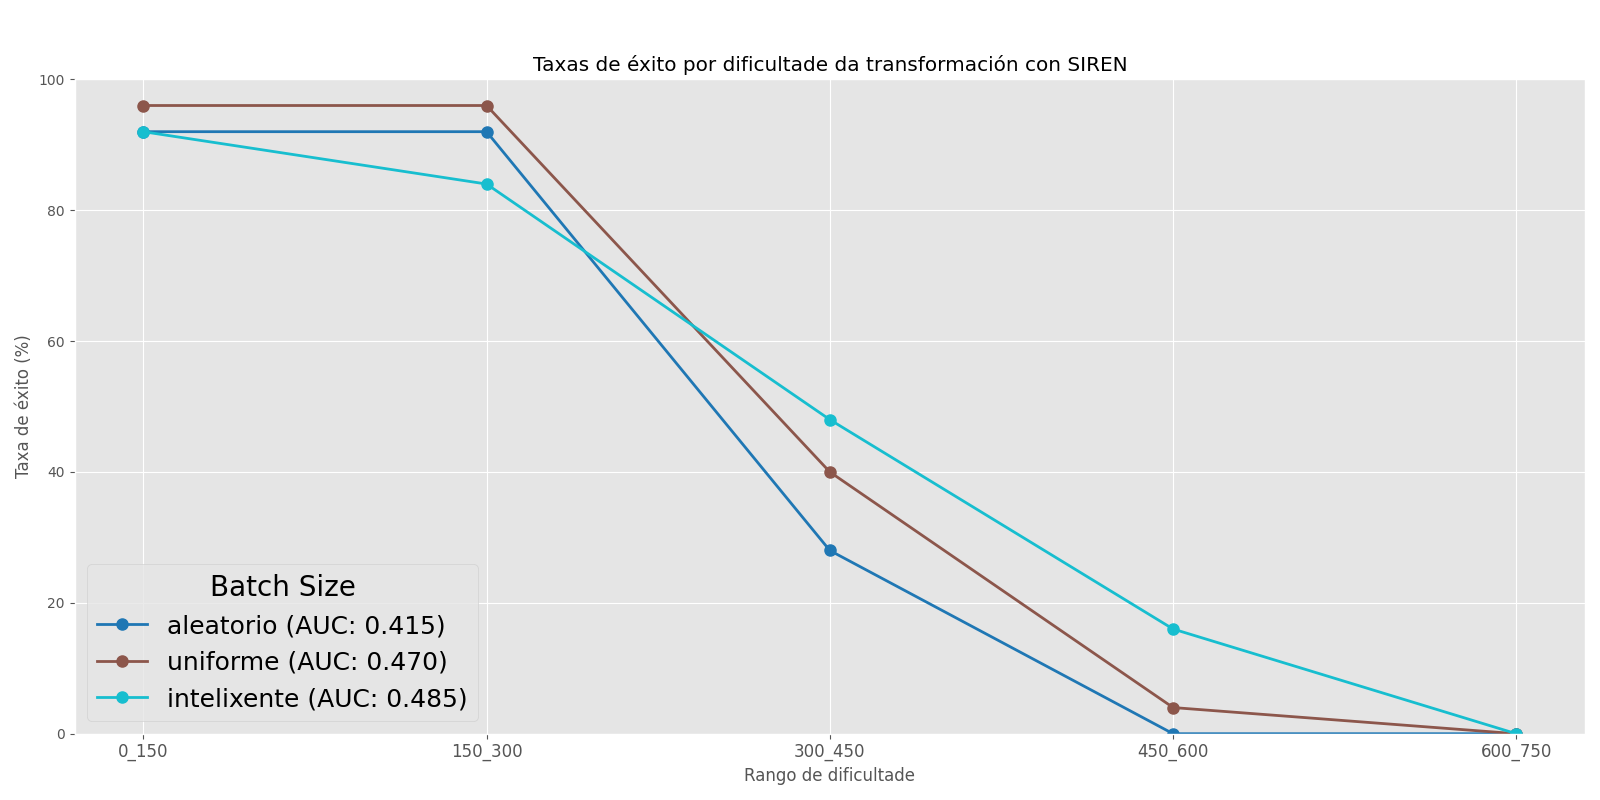
\includegraphics[width=\textwidth]{../imaxes/muestraje/experiment_plot_RFMID_st_SIREN.png}
        \end{column}
    \end{columns}

    \begin{alertblock}{Resultado e Conclusións}
        En contra da hipótese, ningunha das estratexias de mostraxe implementadas ofrece unha vantaxe significativa. Isto indica que a información relevante está suficientemente dispersa, sendo a mostraxe aleatoria axeitada sempre que o tamaño do lote sexa grande dabondo.
    \end{alertblock}

    % NOTAS PARA O PRESENTADOR:
    % - "A primeira estratexia que probei foi unha mostraxe intelixente. A idea era sinxela: en lugar de coller puntos ao chou, centrarse nas zonas con máis detalle, como os vasos."
    % - "Sorprendentemente, como se ve nas gráficas, onde as liñas están practicamente superpostas, isto non tivo ningún impacto relevante."
    % - "A conclusión é que mentres o lote sexa grande, a mostraxe aleatoria xa captura suficiente información."
\end{frame}

\begin{frame}
    \frametitle{Estratexia Desenvolvida: Lotería de Inicialización (I)}
    
    \begin{block}{Hipótese}
        Explorar varias inicializacións de pesos aleatorias e escoller a máis prometedora (baseándose na perda inicial) podería evitar mínimos locais deficientes e mellorar o rendemento final.
    \end{block}
    \vspace{0.5cm}

    \centering
    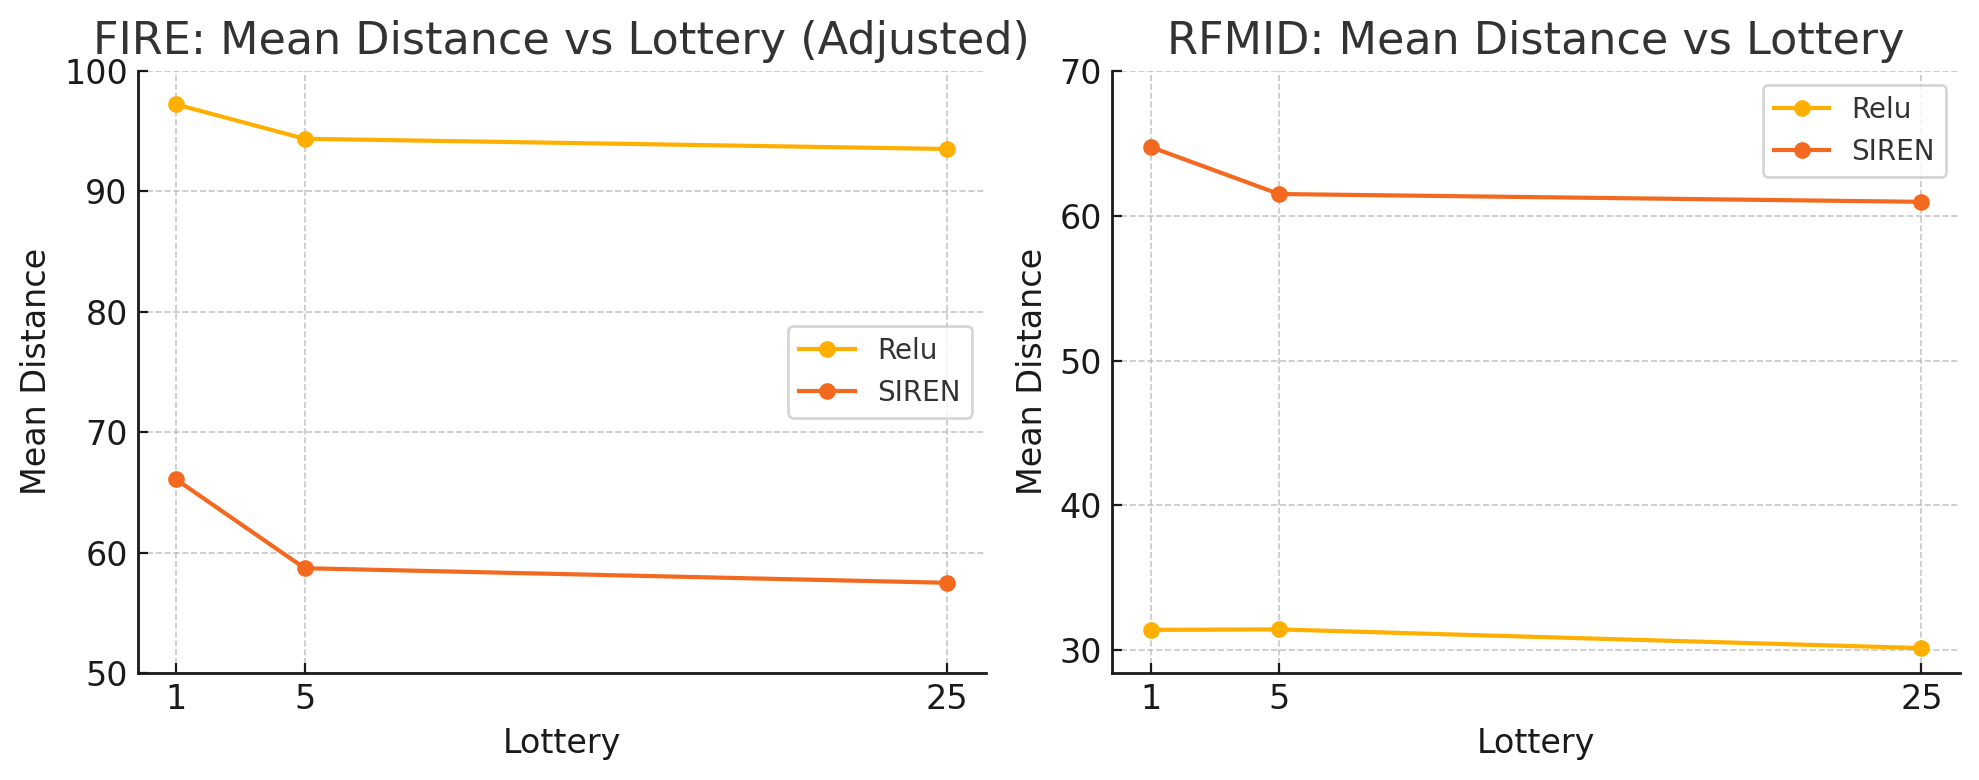
\includegraphics[width=0.7\textwidth]{../imaxes/lottery/lotery.png}
    
    % NOTAS PARA O PRESENTADOR:
    % - "Sabemos que o punto de partida pode influír moito neste tipo de redes. Así que implementei unha 'lotería': probar varias inicializacións e quedar coa mellor."
\end{frame}

\begin{frame}
    \frametitle{Estratexia Desenvolvida: Lotería de Inicialización (II)}
    \begin{alertblock}{Resultado e Conclusión}
        Obsérvase unha mellora marxinal no rendemento. A inicialización ten certo impacto, mais o seu custo computacional adicional pode non xustificar a pequena ganancia.
    \end{alertblock}
    \vspace{0.5cm}

    \centering
    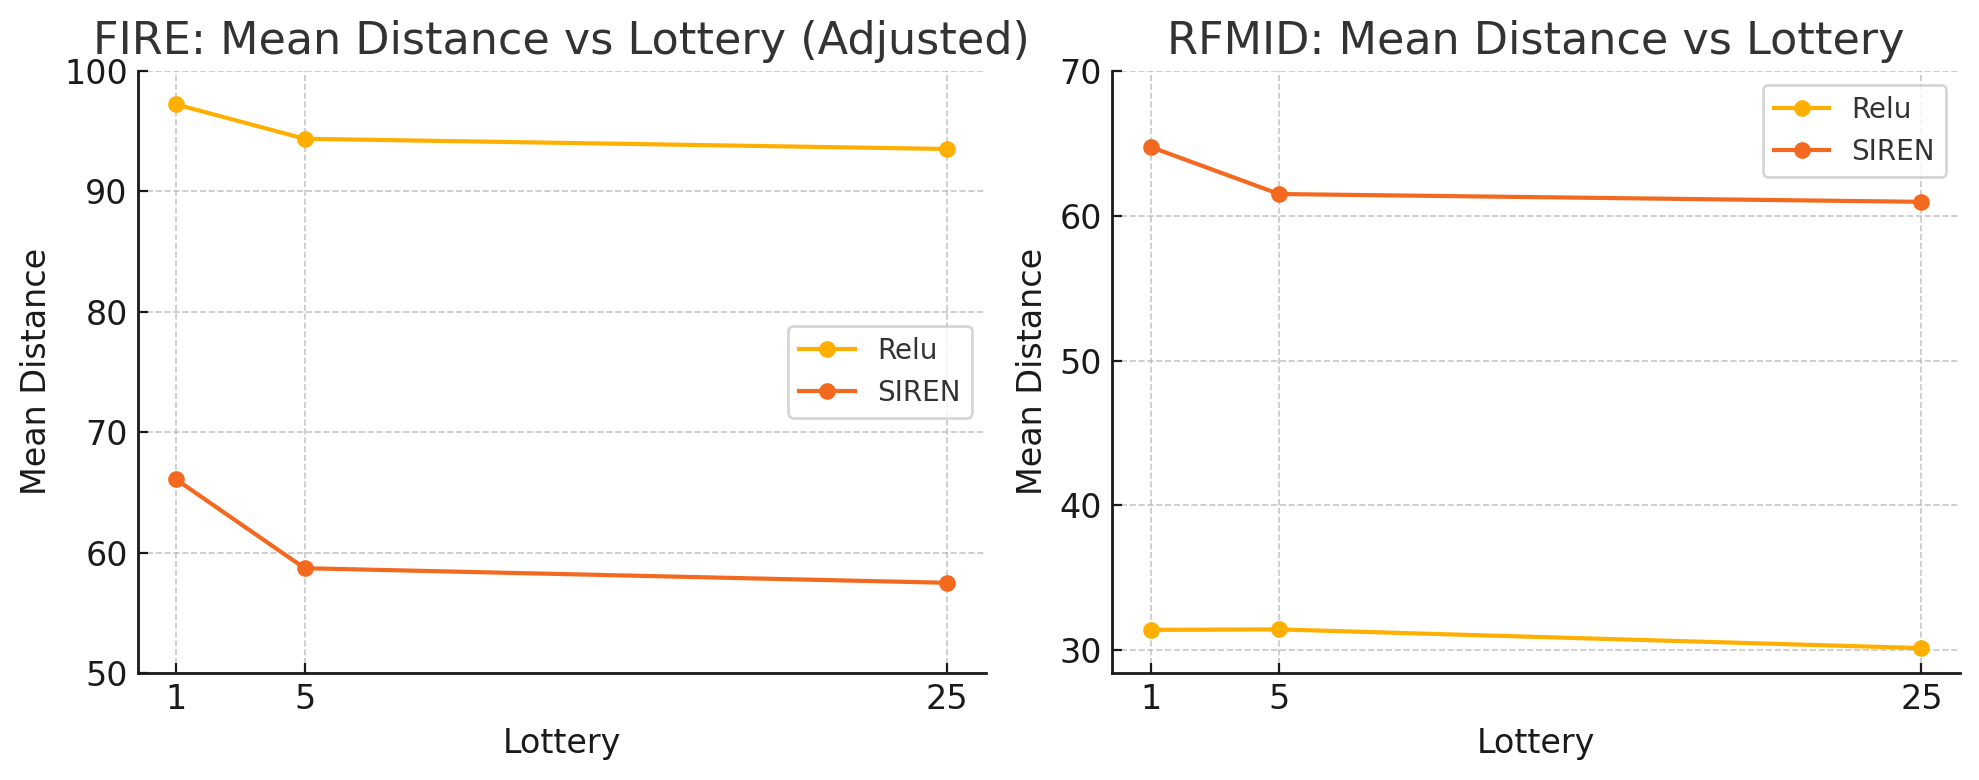
\includegraphics[width=0.7\textwidth]{../imaxes/lottery/lotery.png}
    


    % NOTAS PARA O PRESENTADOR:
    % - "O gráfico mostra que esta estratexia funciona; usar 5 boletos de lotería é mellor que usar só 1. Con todo, a mellora é pequena e usar máis de 5 case non aporta nada."
    % - "Isto confirma que axuda, pero non é unha solución máxica aos problemas fundamentais do rexistro."
\end{frame}

\begin{frame}
    \frametitle{Estratexia Desenvolvida: Axuste Dinámico do Lote (I)}
    
    \begin{block}{Hipótese}
        A rede podería beneficiarse dun adestramento por fases: comezar cun \textit{tamaño de lote} pequeno para aprender a transformación global e despois aumentalo progresivamente para refinar os detalles locais da deformación.
    \end{block}
        \vspace{0.5cm}

    \centering
    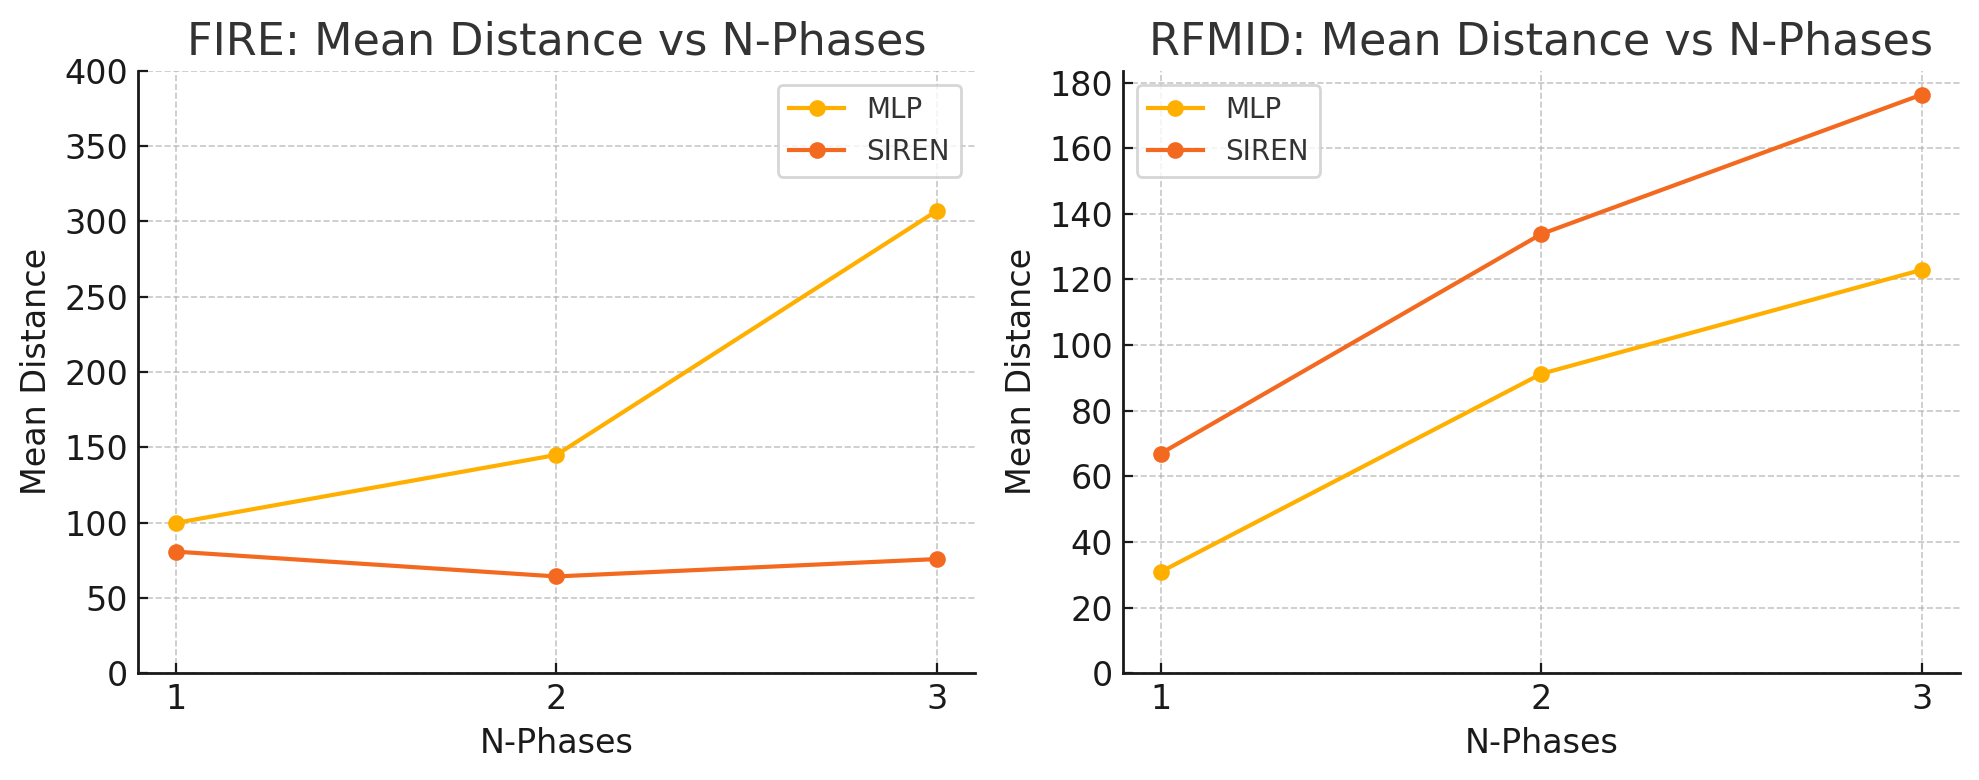
\includegraphics[width=0.7\textwidth]{../imaxes/lottery/nphases.png}
    
    % NOTAS PARA O PRESENTADOR:
    % - "A última idea parecía moi lóxica: ensinar á rede primeiro o 'bosquexo' xeral con poucos puntos, e logo os 'detalles' con moitos puntos."
\end{frame}

\begin{frame}
    \frametitle{Estratexia Desenvolvida: Axuste Dinámico do Lote (II)}
        \begin{alertblock}{Resultado e Conclusión}
        O resultado foi concluínte e contrario á hipótese: esta estratexia resultou ser \textbf{prexudicial}, empeorando o rendemento a medida que se incrementaba o número de fases. Un \textit{tamaño de lote} grande e constante dende o inicio demostrou ser máis estable e eficaz.
    \end{alertblock}
    \vspace{0.5cm}
    \centering
    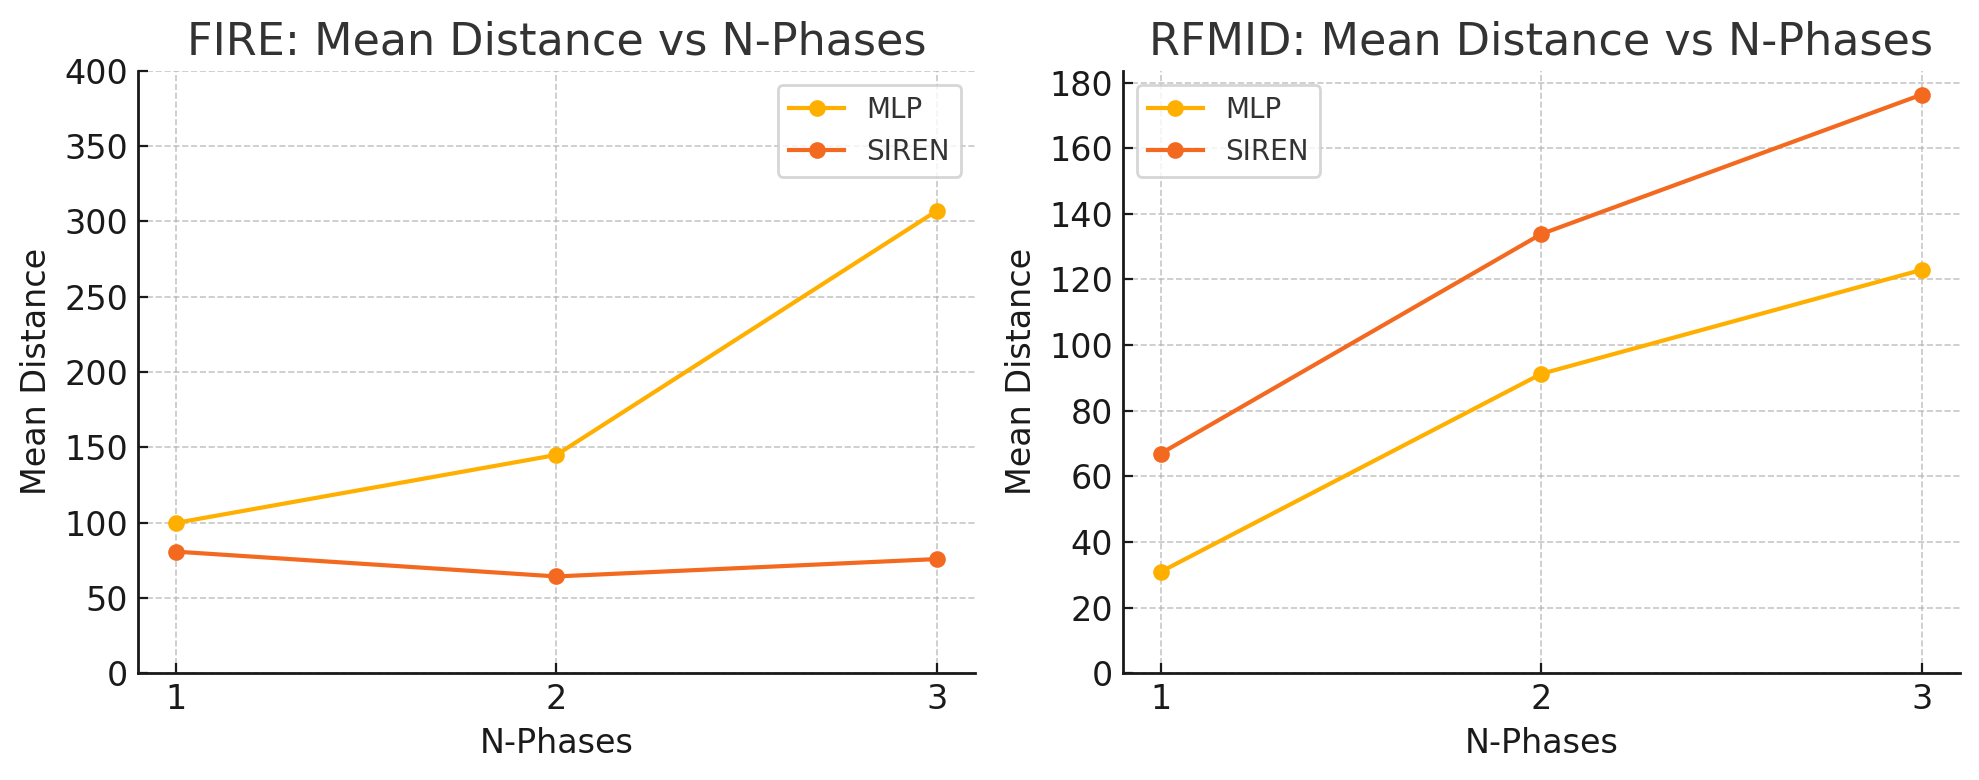
\includegraphics[width=0.7\textwidth]{../imaxes/lottery/nphases.png}
    


    % NOTAS PARA O PRESENTADOR:
    % - "O resultado foi totalmente inesperado: foi contraproducente. Como mostra a gráfica, cantas máis fases usabamos, peor era o resultado."
    % - "A explicación probable é que os lotes pequenos iniciais son demasiado 'ruidosos' e levan á rede por un mal camiño dende o principio, do cal non pode recuperarse. Isto reforza a nosa conclusión anterior: un lote grande dende o inicio é fundamental."
\end{frame}

% ------------------- SECCIÓN 5: CONCLUSIÓNS E TRABALLO FUTURO (VERSIÓN MELLORADA) ---------------------- %
\section{Conclusións e Traballo Futuro}

\begin{frame}
    \frametitle{Conclusións}

    \begin{block}{Resumo}
        O framework IDIR funciona para rexistro de retinografías, pero a súa dependencia só da intensidade dos píxeles limita a robustez clínica.
    \end{block}

    \begin{itemize}
        \item \textbf{ReLU}: boa en transformacións globais e lineais (\textit{RFMID}).
        \item \textbf{SIREN}: eficaz en deformacións locais (\textit{FIRE}), pero require regularización máis coidadosa.
        \item \textbf{Limitación clave}: Falta de correspondencia global; o método é fráxil ante grandes desprazamentos, variacións de aparencia e baixa superposición.
    \end{itemize}

    % NOTAS PARA O PRESENTADOR:
    % - O método adapta o framework, pero non resolve a correspondencia global.
    % - ReLU e SIREN teñen vantaxes distintas.
    % - Os INRs puros non teñen estabilidade nin visión global abonda para rexistro clínico.
    \end{frame}

% --- DIAPOSITIVA DE TRABALLO FUTURO 1: PROPOSTA PRINCIPAL ---
\begin{frame}
    \frametitle{Traballo Futuro (I)}
    
    \begin{block}{Diagnóstico do Problema}
        As nosas conclusións indican que os modelos INR son bós para o \textbf{refinamento local} de deformacións, pero fráxiles para atopar a \textbf{correspondencia global} inicial.
    \end{block}
    
    \begin{alertblock}{Solución Proposta: Enfoque Híbrido}
        Sistema de dous pasos que combina o mellor dos métodos baseados en características e os baseados en aprendizaxe.
    \end{alertblock}
    
    \begin{itemize}
        \item \textbf{Paso 1: Aliñamento global} cun método baseado en puntos clave.
        \item \textbf{Paso 2: Refinamento local} usando o noso modelo INR para axustar detalles finos.
    \end{itemize}
    
    % NOTAS PARA O PRESENTADOR:
    % - "Baseado no noso diagnóstico, a liña de traballo futuro máis prometedora non é mellorar incrementalmente o noso método, senón cambiar o enfoque."
    % - "Propomos un sistema híbrido de dous pasos. No primeiro paso, abordamos a nosa maior debilidade: a correspondencia global. Usamos ferramentas de última xeración como SuperPoint e SuperGlue para atopar un aliñamento inicial robusto, sen importar o desprazamento."
    % - "Unha vez que as imaxes están 'preto', entra en xogo o noso método INR no segundo paso. Agora, o problema é moito máis fácil. O INR non ten que buscar a imaxe, só ten que refinar os detalles, que é onde realmente brilla."
    % - "Este enfoque non só resolve o problema que atopamos, senón que segue a liña dos métodos máis exitosos publicados actualmente no campo."
\end{frame}

% --- DIAPOSITIVA DE TRABALLO FUTURO 2: OUTRAS LIÑAS DE INTERESE ---
\begin{frame}
    \frametitle{Traballo Futuro (II): Mellora da INR}

    \begin{block}{Melloras na arquitectura e regularización}
        \begin{itemize}
            \item \textbf{Consistencia Cíclica:} Adestrar dúas redes (directa e inversa) que se regularicen mutuamente.
            \begin{itemize}
                \item \textit{Vantaxe clave:} Xera unha métrica de certeza da transformación, útil en aplicacións clínicas.
            \end{itemize}
            \item \textbf{Garantir a Invertibilidade:} Empregar arquitecturas baseadas en campos de velocidade ou redes invertibles para obter transformacións máis robustas e realistas.
        \end{itemize}
    \end{block}


\end{frame}

\begin{frame}
    \frametitle{Traballo Futuro (III): Coñecemento Adicional}

    \begin{block}{Incorporación de coñecemento adicional}
        \begin{itemize}
            \item \textbf{Meta-aprendizaxe:} Aprender unha inicialización de pesos óptima a partir dun conxunto de datos para acelerar e estabilizar a converxencia en novas imaxes.
            \item \textbf{Condicionamento por xeometría:} Incorporar coñecemento anatómico previo (ex: segmentación de vasos) para restrinxir o espazo de posibles deformacións.
        \end{itemize}
    \end{block}
    \begin{block}{Melloras no preprocesado}
        \begin{itemize}
            \item Explorar técnicas de preprocesado de imaxes para mellorar a calidade dos datos de entrada e facilitar o rexistro.
        \end{itemize}
    \end{block}
    % NOTAS PARA O PRESENTADOR:
    % - "Ademais da nosa proposta principal, a investigación revelou outras vías interesantes que merecen ser exploradas."
    % - "Poderíamos mellorar o propio motor da rede. Por exemplo, coa consistencia cíclica, adestrar dúas redes á vez para que se 'vixíen' mutuamente, o que estabiliza o adestramento e nos dá unha métrica de confianza."
    % - "Tamén poderíamos incorporar coñecemento externo. O meta-aprendizaxe podería darnos un 'punto de partida' moito mellor para a optimización, e o condicionamento por xeometría usaría mapas anatómicos para guiar a rede."
    % - "Isto demostra que, aínda que o noso proxecto se pecha, abre múltiples e novas portas para futuras investigacións."
\end{frame}


% --- DIAPOSITIVA FINAL ---
\begin{frame}
    \centering
    \Huge
    Grazas pola atención.
    \vspace{1cm}
    % \large
    % Preguntas?
\end{frame}

% --- DIAPOSITIVA DE BACKUP PARA PREGUNTAS ---
\begin{frame}
    \titlepage
\end{frame}

\end{document}